\documentclass[aspectratio=169,10pt]{beamer}
\usetheme{Madrid}
\usecolortheme{seahorse}

\usepackage[utf8]{inputenc}
\usepackage{amsmath,amssymb,amsthm}
\usepackage{graphicx}
\usepackage{listings}
\usepackage{xcolor}
\usepackage{booktabs}
\usepackage{array}
\usepackage{tikz}
\usetikzlibrary{arrows.meta,positioning,shapes,calc}

\graphicspath{{figures/}}

\setbeamertemplate{footline}[frame number]
\setbeamertemplate{navigation symbols}{}

% ---- listings style ----
\lstset{
  basicstyle=\ttfamily\scriptsize,
  numbers=left,
  numberstyle=\tiny\color{gray},
  frame=single,
  backgroundcolor=\color{gray!7},
  keywordstyle=\color{blue}\bfseries,
  commentstyle=\color{green!50!black}\itshape,
  stringstyle=\color{red!60!black},
  showstringspaces=false,
  breaklines=true,
  tabsize=2,
  language=Python
}

% ---- shorthand macros ----
\newcommand{\BB}{\mathbb{B}}
\newcommand{\NN}{\mathbb{N}}
\newcommand{\RR}{\mathbb{R}}
\newcommand{\PP}{\mathbb{P}}
\newcommand{\EE}{\mathbb{E}}
\newcommand{\Acal}{\mathcal{A}}
\newcommand{\Ocal}{\mathcal{O}}
\newcommand{\Ecal}{\mathcal{E}}
\newcommand{\Rcal}{\mathcal{R}}
\newcommand{\Hcal}{\mathcal{H}}
\newcommand{\Mcal}{\mathcal{M}}
\newcommand{\Scal}{\mathcal{S}}
\newcommand{\Ccal}{\mathcal{C}}
\newcommand{\Tcal}{\mathcal{T}}
\newcommand{\CD}{\mathcal{C}_D}
\newcommand{\CDi}[1]{\mathcal{C}_{D_{#1}}}
\newcommand{\PKT}{\mathrm{P}_{\mathrm{KT}}}
\newcommand{\Pkt}{\mathrm{P}_{kt}}
\newcommand{\Pw}{\mathrm{P}_w}

\title[Ch.\ 12: MC-AIXI-CTW]{Monte Carlo AIXI with Context Tree Weighting}
\subtitle{Chapter 12}
\author{Slides based on: Marcus Hutter, Elliot Catt, David Quarel\\
\textit{An Introduction to Universal Artificial Intelligence}, CRC Press, 2024, Chapter 12}
\date{}

\begin{document}

% ============================================================
\begin{frame}
\titlepage
\begin{center}
\small\textit{``The best way to predict your future is to create it.''} --- Peter Drucker
\end{center}
\end{frame}
% ============================================================

\begin{frame}{Outline}
\tableofcontents
\end{frame}

% ============================================================
\section{Learning and Searching}
% ============================================================

\begin{frame}[allowframebreaks]{From AIXI-MDP to a More General Approximation}
\begin{itemize}
\item Chapter 11 introduced \textbf{AIXI-MDP}, an approximation of AIXI that performs a
fixed-depth expectimax search but only over the class of all Markov environments as its
model class. For small $\Ocal=\Acal=\BB$, each environment was encoded as a 4-tuple
$(\theta_{00},\theta_{01},\theta_{10},\theta_{11})$ learned by a KT estimator.
\item This chapter builds a strictly more powerful approximation of AIXI, using as the
model class $\Mcal=\CD$, the set of \emph{all variable-order Markov environments with
context length at most $D$} (recall $D$ is a fixed maximum context depth).
\item We call the resulting agent \textbf{Monte Carlo AIXI with Context Tree Weighting}
(\textbf{MC-AIXI-CTW}). It replaces the two computationally hard parts of AIXI with
tractable approximations:
\begin{itemize}
\item \textbf{Searching}: the exact expectimax operation is replaced by a Monte Carlo
Tree Search (MCTS) variant.
\item \textbf{Learning}: the incomputable Bayes mixture $\xi$ over \emph{all}
semicomputable environments is replaced by a Bayesian mixture over context trees,
computed efficiently using \textbf{Context Tree Weighting (CTW)} (Chapter 4).
\end{itemize}
\item Moving from a limited-depth expectimax search to MCTS lets the agent plan to much
greater depths, and MCTS is asymptotically as good as full expectimax search. Using CTW
for prediction lets the agent model \emph{any} $k$-Markov environment for any $k\le D$,
where $D$ is the maximum depth of the CTW tree.
\end{itemize}
\end{frame}

\begin{frame}{Definition: Action-Observation Search Tree}
\begin{block}{Definition 12.1.1 (Action-observation search tree)}
An \emph{action-observation search tree} is a tree comprised of alternating
\emph{action nodes} and \emph{chance nodes}. Each node is associated with a history $h$.
Additionally, action (resp. chance) nodes store an estimate of the value $\widehat V(h)$
(resp. Q-value $\widehat Q(h,a)$) of the associated history $h$ (resp. $ha$).
\end{block}
\vspace{0.3cm}
\textbf{Plain-English summary.} Think of the tree of everything that \emph{could} happen
from now on: at an action node the agent chooses an action $a$ (white node in
Figure~12.2 below); at the resulting chance node the environment ``rolls the dice'' and
returns an observation/reward pair (black node). $\widehat V(h)$ is the agent's current
best guess at how good the situation described by history $h$ is, and
$\widehat Q(h,a)$ is its best guess at how good it is to take action $a$ having reached
history $h$. Figure~12.1 (next slide) shows how this tree fits into the whole
agent--environment loop of MC-AIXI-CTW.
\end{frame}

\begin{frame}{Figure 12.1: The MC-AIXI-CTW Interaction Loop}
\centering
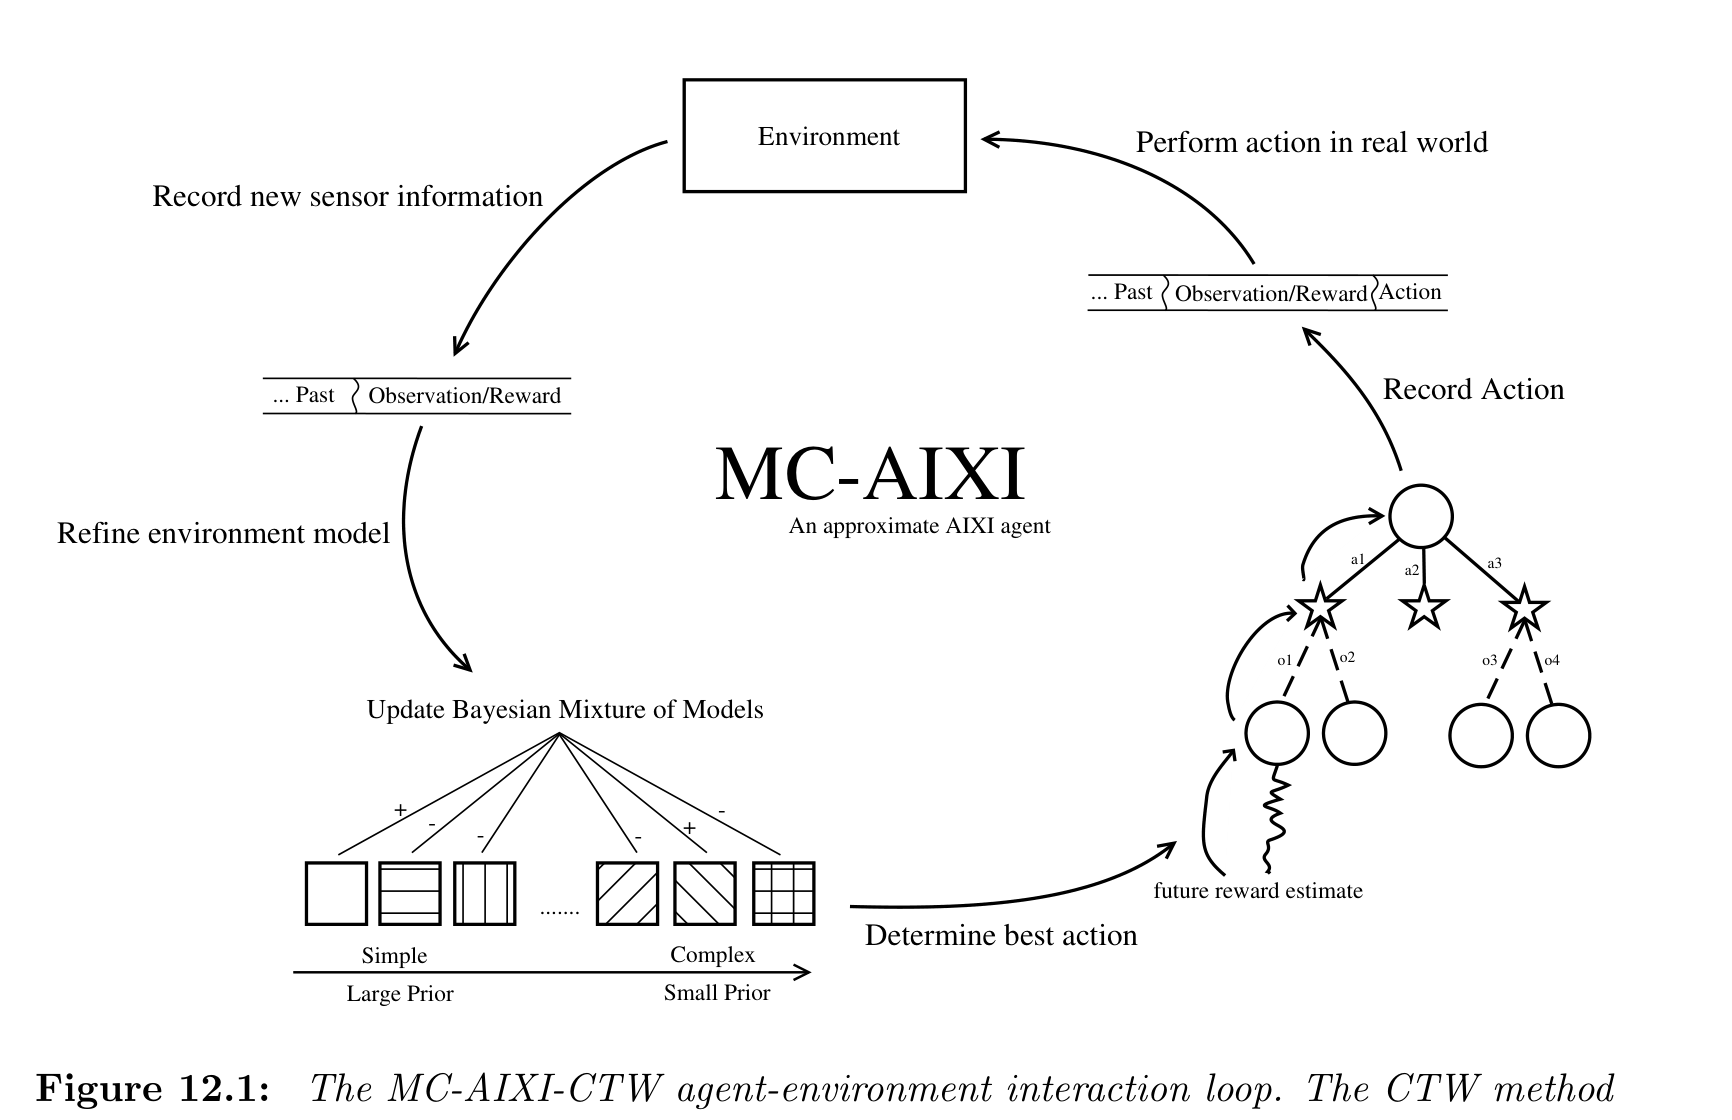
\includegraphics[width=0.92\textwidth]{fig12_1_loop}
\vspace{0.1cm}
\begin{center}
\scriptsize The CTW method provides a Bayesian mixture over models (bottom left: simple,
high-prior models to complex, low-prior models). MCTS is used for action selection
(right), and rollouts are used to estimate the future reward.
\end{center}
\end{frame}

\begin{frame}{Recap: The AIXI Expectimax Operation}
Recall that the action AIXI takes maximizes the (undiscounted) expected value in the
mixture environment $\xi$, given by the expectimax Theorem 7.4.2:
\begin{block}{AIXI Policy (Theorem 7.4.2)}
$$\pi^{\mathrm{AIXI}}(h_{<t}) := \arg\max_{a_t}\sum_{e_t}\cdots
\max_{a_{t+m}}\sum_{e_{t+m}}\left(\sum_{i=t}^{t+m} r_i\right)\sum_{\nu\in\Mcal}
w(\nu|h_{<t})\prod_{k=t}^{t+m}\nu(e_k|h_{<k}a_k)$$
\end{block}
\textbf{Plain-English summary.} $\pi^{\mathrm{AIXI}}$ is the policy (rule for choosing
actions) that AIXI follows. $h_{<t}$ is the history of actions/observations/rewards seen
before time $t$. The agent uses a \emph{forward moving horizon}: it always looks exactly
$m$ steps into the future from the current time step. $e_k$ is a percept
(observation+reward pair) at time $k$; the sums over $e_t,\dots$ range over all possible
future percept sequences, while the $\max_{a_k}$ range over all possible future actions.
$\nu$ (nu) ranges over environments $\nu\in\Mcal$ in the model class, $w(\nu|h_{<t})$ is
the posterior weight (belief) the agent assigns to environment $\nu$ given the history so
far, and $\prod_k \nu(e_k|h_{<k}a_k)$ is the probability that $\nu$ would generate the
imagined future percept sequence. In words: try every action, imagine every possible
consequence, weight each scenario by how much the agent currently believes in the
environment producing it, and pick the action that maximizes expected total reward
$\sum r_i$.
\end{frame}

\begin{frame}{Figure 12.2: Visualizing the Expectimax Tree}
\centering
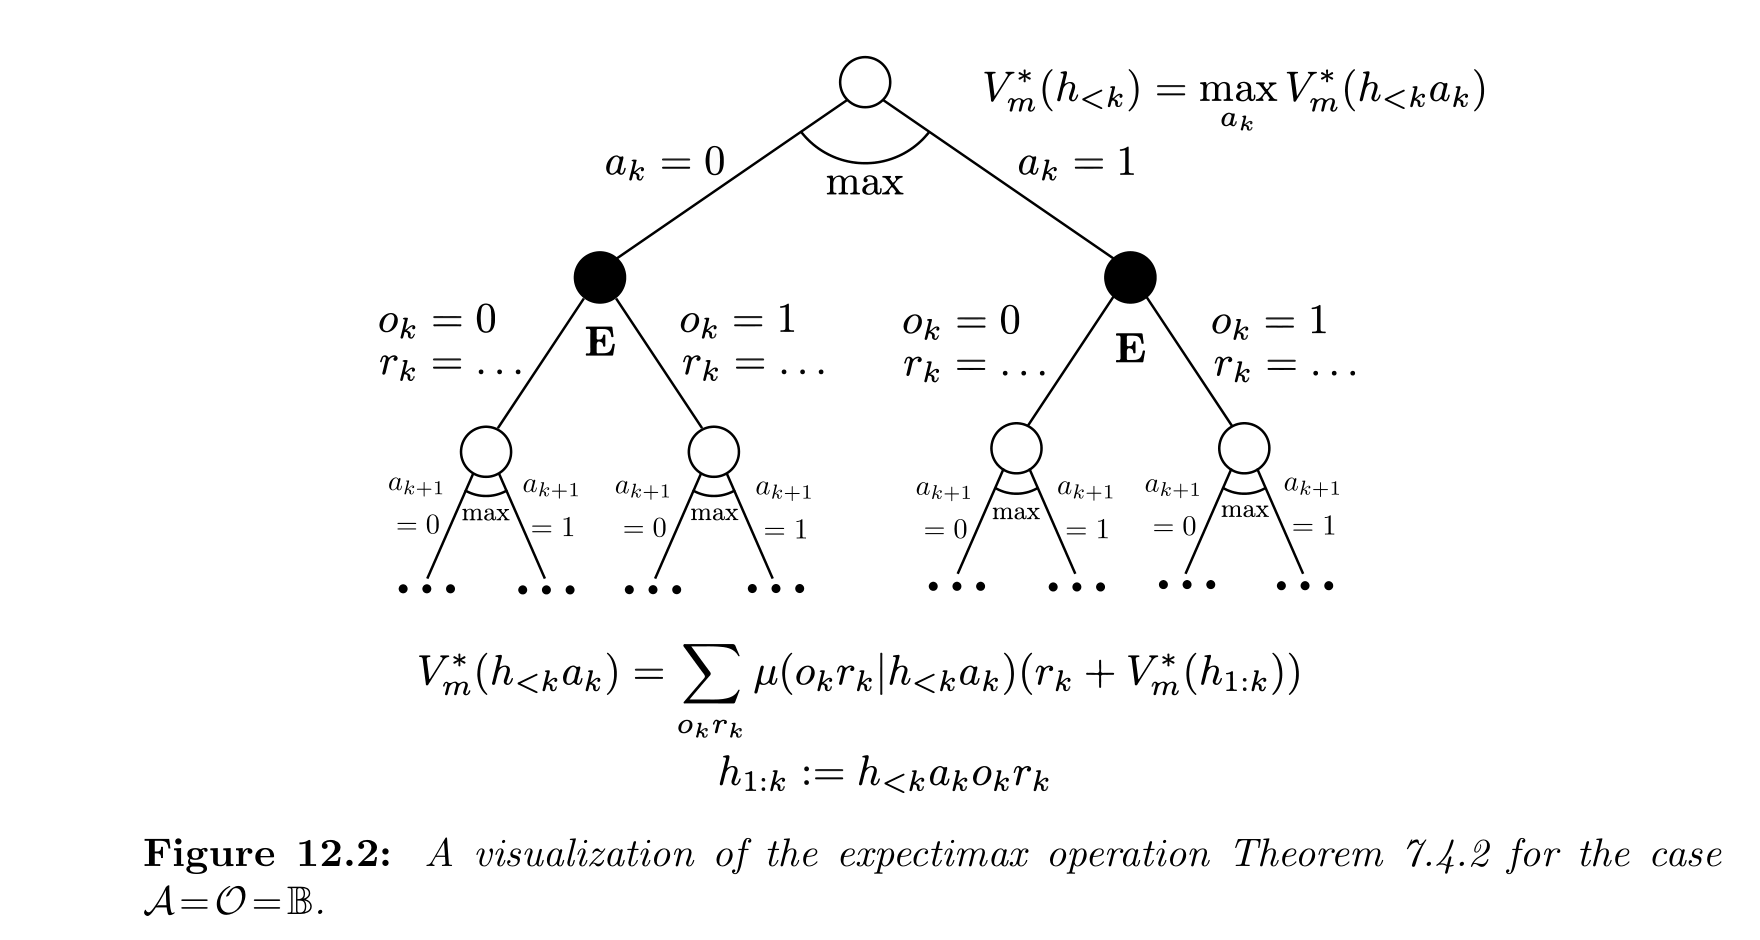
\includegraphics[width=0.95\textwidth]{fig12_2_expectimax}
\vspace{0.2cm}

\small White circles are \emph{action nodes} (the agent picks $a_k\in\{0,1\}$); black
circles are \emph{chance nodes} labelled $\mathbf{E}$ (the environment $\mu$ (mu) responds
with observation $o_k$ and reward $r_k$). The value $V_m^*(h_{<k})$ of a history is the
max over the children's Q-values, and the Q-value of taking action $a_k$ is the
expectation, under the true environment $\mu$, of the immediate reward plus the value of
the continuation $h_{1:k}:=h_{<k}a_ko_kr_k$. This is exactly the Bellman equation
(Theorem 6.7.2) written out as a tree.
\end{frame}

\begin{frame}{The Two Hard Parts of AIXI}
The mixture environment $\xi$ uses the universal prior $2^{-K(\nu)}$ (where $K$ is
Kolmogorov complexity), which is incomputable, and sums over the class $\Mcal$ of
\emph{all} semicomputable chronological semimeasures, which is clearly intractable. The
AIXI agent decomposes roughly into two parts, both problematic to evaluate directly.
\begin{itemize}
\item \textbf{Learning}: computing the Bayesian mixture $\xi$ (based on the history so
far), through which the agent implicitly updates its belief about which environment in
the model class best represents the true environment $\mu$.
\item \textbf{Searching}: using $\xi$ as a current best estimate of $\mu$ to look
forward, considering the actions the agent could choose, the percepts the environment
would respond with, the counter-actions to each percept, and so on up to the planning
horizon $m$. Then the action that maximizes expected cumulative reward is chosen.
\end{itemize}
To compute each of the maximums in the expectimax, we must search through all actions in
$\Acal$ and all percepts in $\Ecal$, requiring $O(|\Acal\times\Ecal|^m)$ time --
intractable for even moderate $m$. We require efficiently computable approximations for
\emph{both} learning and searching to get a practically useful approximation of the AIXI
agent -- this is exactly what MCTS (searching) and CTW (learning) provide.
\end{frame}

% ============================================================
\section{Searching via Monte Carlo Tree Search}
% ============================================================

\begin{frame}{12.2.1 What Is Monte Carlo Tree Search?}
\begin{itemize}
\item Instead of computing the expectimax sums explicitly, we \emph{approximate} them by
\textbf{sampling}: Monte Carlo Tree Search (MCTS) randomly explores paths of the search
tree to estimate the expected value of different histories, rather than brute-forcing the
whole tree.
\item MCTS is an \emph{anytime} search algorithm (it can be terminated at any point in
time with a well-defined return value) that has been very successful in complex domains
such as Go and Backgammon.
\item \textbf{Chess analogy.} Chess has a branching factor of around 35 -- planning 15
moves ahead na\"ively requires exploring $35^{15}\approx 10^{23}$ nodes. A grandmaster
does not search this space exhaustively; instead their intuition tells them which moves
are worth considering and which can be discarded immediately (e.g.\ sacrificing the queen
for a pawn is almost never worth exploring further).
\item MCTS mimics this: from a given position, it decides which actions are worth
exploring, and simulates a potential future using a model of the environment -- much like
a grandmaster mentally ``simulates'' an opponent when planning ahead.
\item MCTS is especially effective in stochastic games with large branching factors
(backgammon, poker), where sampled dice rolls / card deals quickly give a good estimate
of an action's value, and it can easily be parallelized over many rollouts.
\end{itemize}
\end{frame}

\begin{frame}{The Four Steps of MCTS}
\footnotesize
We denote the action-observation search tree as $\Psi$ (Psi). MCTS repeats four steps
while execution time remains:
\begin{enumerate}
\setlength{\itemsep}{0pt}
\item \textbf{Selection}: from the root, $\Psi$ is traversed to a leaf chance node
following a \emph{tree policy}, balancing exploit (known-good moves) vs.\ explore.
\item \textbf{Expansion}: from the leaf chance node, a new unexplored action is selected
and added as a child action node. Only one node is added per iteration.
\item \textbf{Simulation}: from the new action node, a possible outcome is simulated using
a \emph{rollout policy} (a cheap approximate behavior model) and the environment (or the
agent's model of it), up to horizon $m$.
\item \textbf{Backup}: rewards from the simulated trajectory update the value/Q-value
statistics of every node along the path traversed through $\Psi$.
\end{enumerate}
\vspace{-0.35cm}
\centering
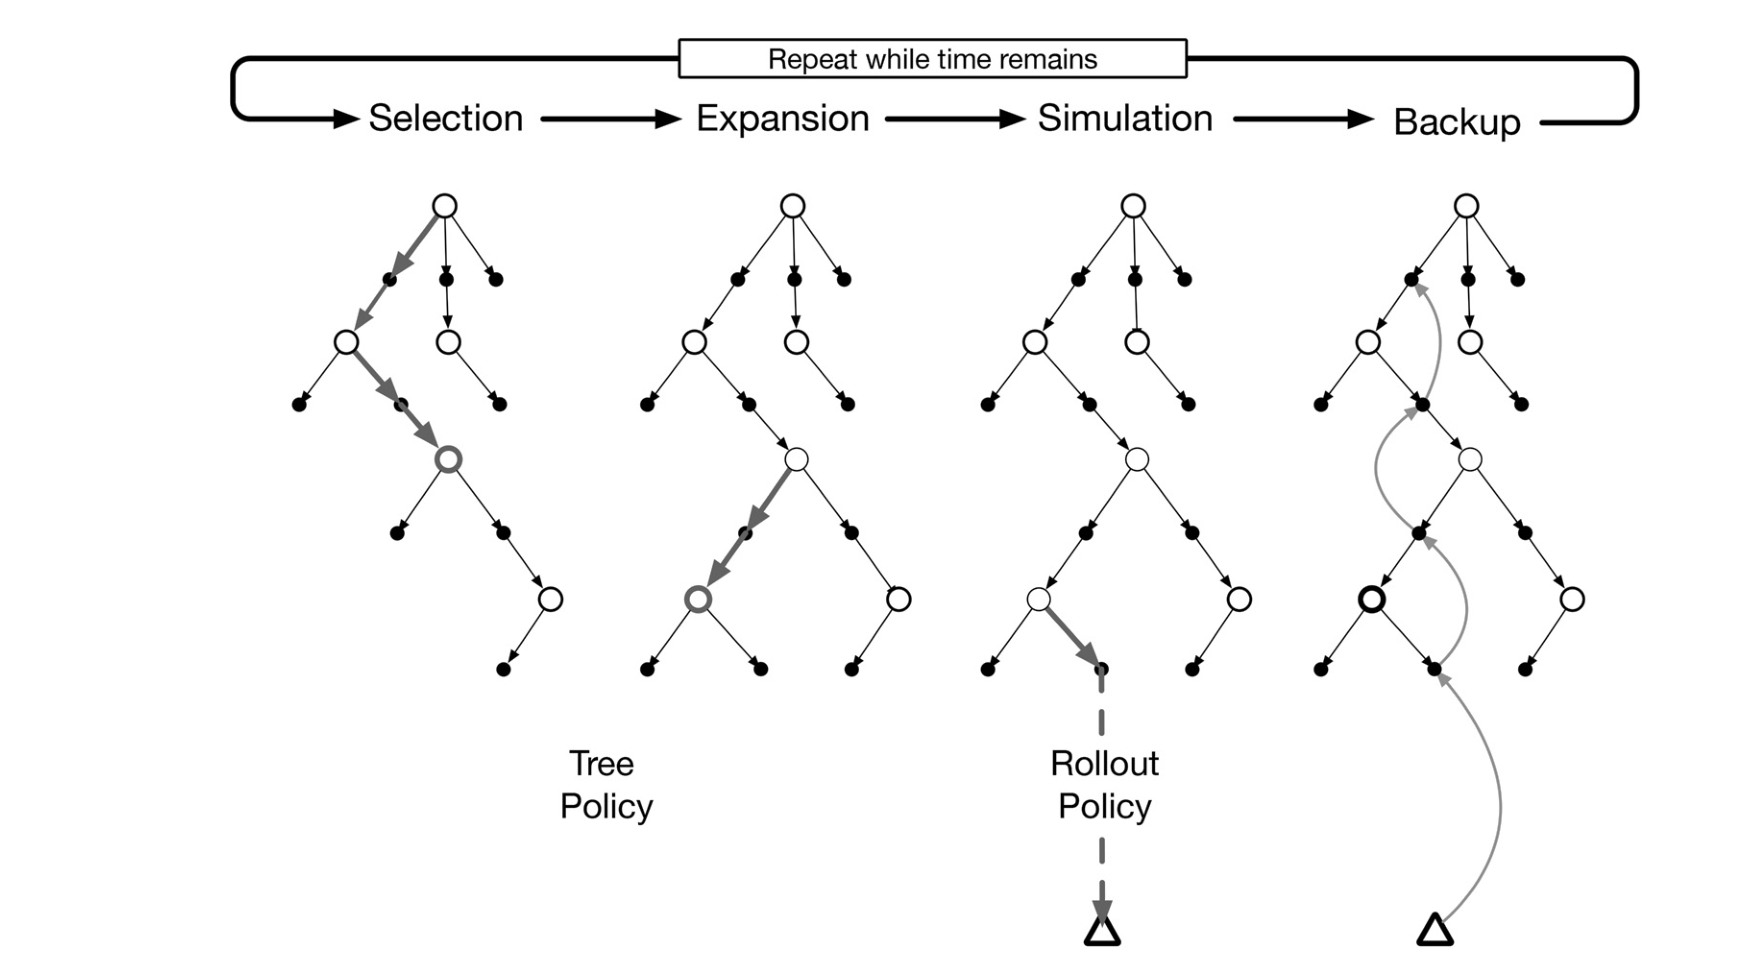
\includegraphics[width=0.58\textwidth]{fig12_3_mcts_steps}
\end{frame}

\begin{frame}{Choosing the Final Action}
\begin{itemize}
\item When execution time has elapsed, MCTS chooses the next action, represented as a
child of the root node, based on the estimated effect of taking that action. The root
still represents the actual present state of the agent--environment interaction.
\item Usually the action with the highest Q-value estimate is taken, but alternatively one
could select randomly with a bias towards high-Q actions, or towards actions visited most
often during backup. A Q-value estimate built from many rollouts should be more accurate
than one built from few, so focusing purely on the current maximum may mean exploiting
before enough exploration has happened.
\item This is the action the agent chooses for interaction with the true environment. The
environment then replies with a percept $e$; MCTS restarts with the updated history
$h:=hae$ as the new root, and the tree can simply be ``walked down'' to the node
associated with $hae$, reusing the existing statistics.
\end{itemize}
\end{frame}

\begin{frame}{12.2.2 MCTS Algorithm: Unspecified Components}
The generic description above leaves several components unspecified, later instantiated
concretely for MC-AIXI-CTW:
\begin{itemize}
\item What statistics are stored in the nodes of $\Psi$.
\item The choice of \emph{tree policy} (the interaction between \textsc{SelectAction} and
\textsc{SimulateAction}).
\item The new action during expansion, and the choice of \emph{rollout policy} (both
inside \textsc{Evaluate}).
\item Updating the node statistics (\textsc{UpdateValue}).
\item Once time has elapsed, choosing the best action from the accumulated statistics
(\textsc{BestAction}).
\end{itemize}
\textbf{Monte Carlo planning} uses a tree $\Psi$ that stores an estimate $\widehat V(h)$ at
each action node and $\widehat Q(h,a)$ at each chance node. It initializes $\Psi$ rooted at
the current history $h$, and repeatedly calls \textsc{Sample} until a time threshold
$t_{\max}$ is exceeded (or a maximum number of simulations is used instead). Each call to
\textsc{Sample} generates a simulated sequence of actions (\textsc{SelectAction}) and
percepts (\textsc{SimulateEnv}). Once time is exceeded, \textsc{BestAction} picks the best
action based on the statistics of $\Psi$. Through repeated simulated interaction, the
agent acquires a better estimate of the Q-values of each history-action pair.
\end{frame}

\begin{frame}{Algorithm 12.1: Monte Carlo Planning}
\begin{block}{Algorithm 12.1 Monte Carlo planning$(h,m,t_{\max})$ [KS06]}
\textbf{Input:} History $h$; Horizon $m$; Timeout time $t_{\max}$\\
\textbf{Output:} An action $a$
\begin{enumerate}
\setcounter{enumi}{0}
\item[1:] $\Psi:=$ action-observation tree starting at $h$
\item[2:] \textbf{while} running time less than $t_{\max}$ \textbf{do}
\item[3:] \quad Sample$(\Psi,h,m)$
\item[4:] \textbf{return} BestAction$(\Psi,h)$
\end{enumerate}
\end{block}
\vspace{0.3cm}
\textbf{Sample (Algorithm 12.2)} computes a recursive function taking as input the tree
$\Psi$, the current history $h$, and the planning horizon $m$. The recursion ends when $m$
reaches $0$, at which point \textsc{Evaluate} estimates the value of the (non-terminal)
history. Otherwise, \textsc{Sample} generates a new action $a$ via \textsc{SelectAction},
and a new percept $(o,r)$ given $a$ via \textsc{SimulateEnv}; it recursively calls itself
on $h':=haor$ with horizon $m-1$, adds the resulting value to reward $r$, updates the
Q-value of $(h,a)$ via \textsc{UpdateValue}, and returns the estimate.
\end{frame}

\begin{frame}{Algorithms 12.2--12.3: Sample and UpdateValue}
\begin{columns}[T]
\begin{column}{0.5\textwidth}
\begin{block}{Algorithm 12.2 Sample$(\Psi,h,m)$}
\textbf{Input:} Tree $\Psi$; history $h$; horizon $m$\\
\textbf{Output:} Q-value estimate $q$
\footnotesize
\begin{enumerate}
\item[1:] \textbf{if} $m=0$ \textbf{then}
\item[2:] \quad \textbf{return} $0$
\item[3:] \textbf{else}
\item[4:] \quad $a:=$SelectAction$(\Psi,h,m)$
\item[5:] \quad $(o,r):=$SimulateEnv$(\Psi,h,a)$
\item[6:] \quad $h':=haor$
\item[7:] \quad $q:=r+$Sample$(\Psi,h',m-1)$
\item[8:] \quad UpdateValue$(\Psi,h,a,q)$
\item[9:] \textbf{return} $q$
\end{enumerate}
\end{block}
\end{column}
\begin{column}{0.5\textwidth}
\begin{block}{Algorithm 12.3 UpdateValue$(\Psi,h,a,q)$}
\textbf{Effect:} update Q-value estimate on node $ha$
\footnotesize
\begin{enumerate}
\item[1:] $\Psi(ha).Q := \dfrac{q+\Psi(ha).N\times\Psi(ha).Q}{\Psi(ha).N+1}$
\item[2:] $\Psi(ha).N := \Psi(ha).N+1$
\end{enumerate}
\end{block}
\end{column}
\end{columns}
\vspace{0.3cm}
\textbf{Plain-English summary.} $q$ is the reward-to-go estimate that a single simulated
rollout produced; $N$ counts how many rollouts have passed through node $ha$; $Q$ is a
running \emph{average} of all $q$'s seen so far, updated incrementally so we never need to
store the individual samples.
\end{frame}

\begin{frame}{How Well Does Sample Perform?}
The performance of \textsc{Sample} depends on two things:
\begin{itemize}
\item \textbf{Accuracy of \textsc{SimulateEnv}.} For known environments, we sample
$e\sim\mu(\cdot|ha)$ directly. For unknown environments (an agent exploring a maze, or
playing a game against an opponent whose strategy is unknown) the agent needs a model of
the environment to sample from -- performance is then tied to how good that model is. Many
MCTS variants sample from an internal model and then update it once a true percept is
received.
\item \textbf{The \textsc{SelectAction} function (also called the rollout policy).} The
agent obviously cannot use MCTS itself to choose the rollout action (that would cause
infinite regress), so we need a cheap, sensible rollout policy: an inexpensive estimate of
what action the agent would take. In vanilla Monte Carlo planning, the rollout policy just
picks uniformly at random. The \emph{greedy} approach picks the action currently believed
best, but can lead to suboptimal play if the current Q-value estimates are inaccurate.
More advanced techniques learn a model (e.g.\ a neural network) of the agent's own
behavior, and sample the rollout policy from that model.
\end{itemize}
\textbf{\textsc{UpdateValue}} is called whenever a recursive \textsc{Sample} call returns
a value; it combines the new Q-value sample with the statistics already collected at the
chance node $ha$, and has no return value (only a side effect on the tree).
\end{frame}

\begin{frame}{12.2.3 Bandits: A Simpler Sub-problem}
Before explaining UCT, we motivate it with \emph{bandit} problems, a simpler subclass of
Markov Decision Processes that still have exploration--exploitation trade-offs. The name
comes from ``one-armed bandit'', a slot machine.
\begin{block}{Definition 12.2.1 (Bandit)}
Given a set of actions $\Acal$ and rewards $\Rcal$, a \emph{bandit} environment is a
stochastic function $\mu:\Acal\to\Delta\Rcal$.
\end{block}
\textbf{Plain-English summary.} $\Delta\Rcal$ denotes the set of probability
distributions over the reward set $\Rcal$; so a bandit just maps each action to a
(possibly random) reward, with no notion of state or observation -- the agent is always
``in the same situation''. Equivalently, a bandit is an MDP with a single state
$\Scal=\{s\}$. The interaction history is $a_1r_1a_2r_2a_3r_3\ldots a_mr_m$ up to length
$m$. The agent wants to maximize the sum of rewards over a fixed horizon. Performance is
often measured by \emph{regret}: the gap between the expected reward the agent obtains and
that of the optimal policy $\pi^*$ (or the best policy from a reference class $\Pi$).
Despite the apparent simplicity, bandits are still non-trivial: the expected value of
each action is unknown, so the agent must trade off exploiting the best-known action
against exploring to improve its estimates.
\end{frame}

\begin{frame}{Estimating Action Values, and $\varepsilon$-Greedy}
If the agent knew the true expected reward $q^*(a):=\EE_\mu[r_t|a_t=a]$ for every action,
it could just always pick $a^*:=\arg\max_a q^*(a)$. Instead, it estimates
$\widehat Q_t(a)\approx q^*(a)$ from the rewards obtained so far:
$$\widehat Q_t(a) \;=\; \frac{\sum_{i=1}^{t-1} r_i\,[\![a_i=a]\!]}{\sum_{i=1}^{t-1}[\![a_i=a]\!]}$$
\textbf{Plain-English summary.} $[\![a_i=a]\!]$ is $1$ if action $a$ was chosen at step
$i$ and $0$ otherwise, so $\widehat Q_t(a)$ is simply the average reward observed so far
whenever action $a$ was played. An agent playing \emph{greedily} w.r.t.\ $\widehat Q_t$
(always taking $\arg\max_a\widehat Q_t(a)$) may never learn to abandon a suboptimal action
that merely \emph{looked} good early on -- it stops collecting information once it
believes it knows the best action.
$$a_t^{\varepsilon\text{-greedy}} = \begin{cases}
\text{uniformly random } a\in\Acal & \text{probability } \varepsilon\\
\arg\max_{a\in\Acal}\widehat Q_t(a) & \text{probability } 1-\varepsilon
\end{cases}$$
\textbf{Plain-English summary.} $\varepsilon$ (epsilon) is a fixed exploration
probability: with probability $\varepsilon$ the agent explores completely at random, and
otherwise exploits the current best-known action. Eventually the agent chooses the best
action with probability $1-\frac{|\Acal|-1}{|\Acal|}\varepsilon$. Too small an
$\varepsilon$ means slow learning; too large means the agent keeps choosing known-bad
actions. $\varepsilon$-greedy is unsophisticated: it explores uniformly, potentially
wasting time on actions already known to be poor.
\end{frame}

\begin{frame}{Upper Confidence Bound (UCB)}
A more sophisticated method focuses exploration on actions whose current value estimate
$\widehat Q_t(a)$ is \emph{uncertain}.
\begin{block}{UCB Q-value (Eq.\ 12.2.2)}
$$Q_t^{\mathrm{UCB}}(a) := \begin{cases}
\widehat Q_t(a) + c\sqrt{\dfrac{\ln(t)}{N_t(a)}} & N_t(a)>0\\[4pt]
\infty & N_t(a)=0
\end{cases}$$
\end{block}
\textbf{Plain-English summary.} $N_t(a):=\sum_{i=1}^{t-1}[\![a_i=a]\!]$ counts how many
times $a$ has been chosen before step $t$; $c>0$ is a hyperparameter controlling how
strong the exploration bonus is. The agent then plays
$a_t^{UCB}:=\arg\max_a Q_t^{\mathrm{UCB}}(a)$. Intuitively, if action $a$ has been tried
$N_t(a)$ times, the relative error $\frac{Q_t(a)-\widehat Q_t(a)}{Q_t(a)}$ is proportional
to $\frac{1}{\sqrt{N_t(a)}}$; adding a bonus of this size encourages visiting actions that
are either genuinely good, or whose value is still uncertain. Assigning a value of
$\infty$ when $N_t(a)=0$ both avoids a divide-by-zero \emph{and} forces the agent to try
every action at least once before anything else.
\end{frame}

\begin{frame}[fragile]{Python: $\varepsilon$-Greedy vs.\ UCB on a Toy Bandit}
\begin{lstlisting}
import numpy as np
rng = np.random.default_rng(0)

# Two-armed bandit: a0 gives reward 1 (always, mean 1);
# a1 gives reward 5 w.p. 0.3, else 0 (mean 1.5, the better arm)
def reward(a):
    return 1.0 if a == 0 else (5.0 if rng.random() < 0.3 else 0.0)

def run(policy, T=200, eps=0.2, c=2.0):
    N = np.zeros(2); Q = np.zeros(2)
    for t in range(1, T + 1):
        if policy == "eps-greedy":
            a = rng.integers(2) if rng.random() < eps else int(np.argmax(Q))
        else:  # UCB
            score = [np.inf if N[i] == 0 else
                     Q[i] + c * np.sqrt(np.log(t) / N[i]) for i in range(2)]
            a = int(np.argmax(score))
        r = reward(a)
        N[a] += 1; Q[a] += (r - Q[a]) / N[a]
    return Q, N

for policy in ["eps-greedy", "UCB"]:
    Q, N = run(policy)
    print(f"{policy:11s}  Q-hat={np.round(Q,2)}  N={N}")
# eps-greedy  Q-hat=[1.02 1.62]  N=[ 90 110]   (varies run to run)
# UCB         Q-hat=[1.0  1.58]  N=[ 46 154]   (UCB commits to the better arm faster)
\end{lstlisting}
\end{frame}

\begin{frame}{12.2.4 The UCT Algorithm}
\textbf{Upper Confidence Trees (UCT)} extends Monte Carlo planning (Algorithm 12.1) by
replacing uniform action selection with a modified UCB rule.
\begin{itemize}
\item \textbf{Random} action selection is inefficient: it wastes computation exploring
actions that are obviously bad a priori (e.g.\ moving a chess piece into certain capture).
\item \textbf{Greedy} action selection exploits too early, before adequate statistics are
collected, getting stuck with overconfident value estimates.
\end{itemize}
UCT balances the two: the UCT-value has an exploration bonus proportional to
$\frac{1}{\sqrt N}$, where $N$ is the number of times the action has been sampled. If an
action has seldom been taken, its Q-value estimate is uncertain, so the bonus is large,
encouraging the agent to explore it.
\begin{block}{Definitions 12.2.3--12.2.4 (Visit count \& UCT action selection)}
The \emph{visit count} $N(h)$ of history $h$ is the number of times $h$ has been sampled
by UCT; $N(ha)$ similarly counts visits to the history-action pair. The action chosen by
UCT is
$$a_{UCT}(h) := \arg\max_{a\in\Acal} Q_{UCT}(h,a),\qquad
Q_{UCT}(h,a):=\begin{cases}
\dfrac{1}{m}\widehat Q(h,a) + C\sqrt{\dfrac{\ln N(h)}{N(ha)}} & N(ha)>0\\[4pt]
\infty & N(ha)=0
\end{cases}$$
(ties broken arbitrarily.)
\end{block}
\end{frame}

\begin{frame}{Interpreting the UCT Formula}
\begin{itemize}
\item $\widehat Q(h,a)$ is the current unbiased frequentist estimate (Algorithm 12.3) of
the Q-value of history $h$, action $a$; dividing by $m$ (the planning horizon) rescales it
to be comparable to the bonus term, since rewards accumulate over up to $m$ steps.
\item $C\in\RR$ is a positive exploration--exploitation hyperparameter. Small $C$ makes
the agent focus on exploiting its current best-looking actions, producing a deep but
narrow tree; large $C$ incentivizes exploration, producing a shallow but broad tree.
\item Assigning $\infty$ when $N(ha)=0$ forces UCT to always prioritize a never-before-
chosen action $a$ over anything else, exactly as with plain UCB.
\item The logarithmic term $\ln N(h)$ in the exploration bonus is crucial: it ensures the
agent chooses \emph{every} action infinitely often (even ones with low current Q-value),
though at a logarithmically decreasing rate. This is what guarantees convergence, both in
theory and in practice.
\end{itemize}
The \textsc{SelectAction} part of MCTS matters because we don't want the search tree to go
down paths that give low reward, but we also want to explore history-action pairs we've
rarely visited -- exactly the same exploration/exploitation trade-off as in the bandit
case, now applied recursively at every node of the tree.
\end{frame}

\begin{frame}{Example 12.2.5: Upper Confidence Bounds for a Bandit}
\small
\begin{columns}[T]
\begin{column}{0.32\textwidth}
\centering
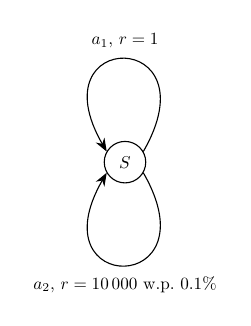
\begin{tikzpicture}[>=Stealth, scale=0.62, every node/.style={scale=0.62}]
\node[circle,draw,minimum size=0.85cm] (S) {$S$};
\draw[->] (S.30) to[out=60,in=120,looseness=10] node[above,yshift=1mm]{$a_1,\,r=1$} (S.150);
\draw[->] (S.330) to[out=-60,in=-120,looseness=10] node[below,yshift=-1mm]{$a_2,\,r=10\,000$ w.p.\ $0.1\%$} (S.210);
\end{tikzpicture}
\end{column}
\begin{column}{0.68\textwidth}
Consider this (trivially) Markov decision process, technically a bandit: a single state
$S$, both actions lead back to $S$, and the history is irrelevant, so $h$ is always empty.
Action $a_1$ \emph{always} returns reward $1$. Action $a_2$ returns reward $10\,000$ with
probability $10^{-3}$, else $0$ -- an \emph{expected} return of $r=10$. Hence the optimal
policy is to \emph{always} choose $a_2$.
\end{column}
\end{columns}
\vspace{0.15cm}
Now suppose the agent follows a UCT-like rule but with the log term \textbf{removed}:
$$a_{UCT'}(h):=\arg\max_a Q_{UCB'}(h,a),\quad
Q_{UCB'}(h,a):=\begin{cases}\frac1m\widehat Q(h,a)+C\sqrt{\dfrac1{N(ha)}} & N(ha)>0\\
\infty & N(ha)=0\end{cases}$$
which is the same as $a_{UCT}$ but without $\ln N(h)$.
\end{frame}

\begin{frame}{Example 12.2.5 (continued): Why $\ln N(h)$ Matters}
\small
Unless the agent got particularly lucky and observed $r=10\,000$ from $a_2$ soon, it will
choose $a_2$ only finitely many times and then always choose $a_1$ thereafter. Assume
$\widehat Q(h,a_1)=1$ (its true value) and, for a moment, $\widehat Q(h,a_2)=0$ (as $a_2$
has not yet returned a non-zero reward). Then:
$$Q_{UCB'}(h,a_1) = \frac{\widehat Q(h,a_1)}{m}+C\sqrt{\frac{1}{N(ha_1)}} > \frac1m,
\qquad
Q_{UCB'}(h,a_2) = \frac{\widehat Q(h,a_2)}{m}+C\sqrt{\frac1{N(ha_2)}}=C\sqrt{\frac1{N(ha_2)}}$$
So once $N(a_2)>(Cm)^2$, we get $\frac1m>C\sqrt{1/N(ha_2)}$ and the agent \textbf{never
again} chooses $a_2$ -- it never learns the optimal policy!

For $C=2$, $m=10$: we need $N(a_2)>400$, and there is a $\approx(1-0.001)^{400}\approx
67\%$ chance $a_2$ never returns a reward over $400$ interactions.

\textbf{Adversarial construction.} Fix $\delta>0$. Choose
$\varepsilon=1-\exp\!\big(\frac{\ln\delta}{C^2m^2}\big)$ and add an action returning reward
$10/\varepsilon$ with probability $\varepsilon$ (expected value still $10$). Then
$$\PP(a_2\text{ finitely often}) \;\ge\; \PP(a_2\text{ returns } 0 \text{ over } C^2m^2
\text{ trials}) \;=\; (1-\varepsilon)^{C^2m^2} \;=\; \delta.$$
So for \emph{any} fixed horizon $m$ and exploration constant $C$, we can build an
adversarial bandit where $a_{UCT'}$ fails to find the optimal action with probability at
least $\delta$ -- no matter how small $\delta$ is. This is exactly the failure mode the
$\ln N(h)$ term is designed to prevent.
\end{frame}

\begin{frame}{Why the Logarithmic Bonus Is the Right Fix}
\begin{itemize}
\item One could try other exploration schedules -- a decaying $\varepsilon_t$-greedy, or a
\emph{Boltzmann distribution} (sampling $a$ with probability
$\propto\exp(\widehat Q(h,a)/T)$, with ``temperature'' $T$ controlling how sharp the
distribution is, analogous to statistical physics: a very cold system, $T\to0$, barely
moves, while a hot one, $T\to\infty$, wiggles a lot). But these all have their own
problems: decaying schedules are hard to tune for arbitrary environments, and choosing the
right cooling rate for $T$ is itself an unsolved sub-problem.
\item The universal solution is to add $\ln N(h)$ to the numerator of the exploration
bonus. This guarantees every action is explored at least logarithmically often (hence
infinitely often over an infinite horizon), so the agent eventually samples $a_2$ enough
times to learn it is the better action.
\item One could use other functions in $o(\sqrt n)$, such as $\ln^2 N(h)$ or
$\sqrt[3]{N(h)}$, but it can be shown that $\ln N(h)$ is \emph{optimal} in the sense of
giving the best bound on the \emph{worst-case regret} -- the largest possible gap between
the expected reward of $\pi_{UCT}$ and that of the optimal policy $\pi^*_\mu$, over any
choice of environment $\mu$.
\end{itemize}
\end{frame}

\begin{frame}{Illustration: UCT vs.\ UCB$'$ on Example 12.2.5}
\centering
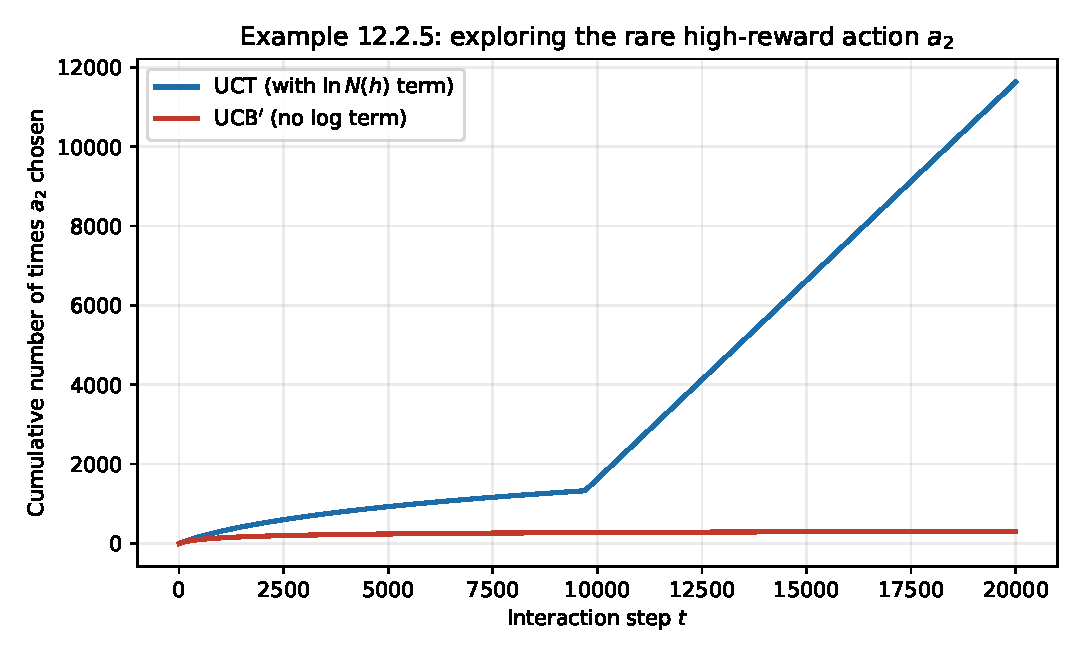
\includegraphics[width=0.62\textwidth]{fig_ucb_vs_uct_bandit}

\footnotesize A simulation of both rules on Example~12.2.5's bandit ($C=2$, $m=10$,
$20\,000$ steps). \textbf{UCT} (blue, with the $\ln N(h)$ term) keeps sampling the rare
high-reward action $a_2$ throughout the run. \textbf{UCB$'$} (red, without the log term)
samples $a_2$ a bounded number of times and then stops exploring it altogether, exactly as
predicted by the argument on the previous slide.
\end{frame}

\begin{frame}[fragile]{Python: Reproducing Example 12.2.5 Numerically}
\begin{lstlisting}
import numpy as np
rng = np.random.default_rng(1)

def simulate(use_log, T=20000, C=2.0, m=10):
    N = np.zeros(2); Q = np.zeros(2)
    picks_a2 = 0
    for t in range(1, T + 1):
        scores = np.empty(2)
        for a in range(2):
            if N[a] == 0:
                scores[a] = np.inf
            else:
                bonus = C * np.sqrt((np.log(t) if use_log else 1.0) / N[a])
                scores[a] = Q[a] / m + bonus
        a = int(np.argmax(scores))
        r = 1.0 if a == 0 else (10000.0 if rng.random() < 1e-3 else 0.0)
        N[a] += 1; Q[a] += (r - Q[a]) / N[a]
        picks_a2 += (a == 1)
    return N[1], picks_a2  # final visit count of a2, total times a2 was picked

for use_log, name in [(False, "UCB' (no log)"), (True, "UCT (with log)")]:
    N_a2, picks = simulate(use_log)
    print(f"{name:16s}: N(a2) after 20000 steps = {int(N_a2):5d}")
# UCB' (no log)  : N(a2) after 20000 steps ~   30   (gets stuck avoiding a2 early on)
# UCT (with log) : N(a2) after 20000 steps ~ 3000+  (keeps exploring a2 throughout)
\end{lstlisting}
This matches Figure~12.9's illustration above: UCT keeps sampling the rare high-reward
action $a_2$ throughout, while the log-free variant can get permanently stuck on $a_1$.
\end{frame}

\begin{frame}{Convergence of UCT}
A general theoretical result [KS06] shows that the estimate of the expectimax value
produced by UCT, $V_{UCT}(h):=V^{\pi_{UCT}}(h)$, \textbf{converges in probability} to the
optimal expectimax value $V^*(h)$, with respect to the implied distribution
$\mu^{\pi_{UCT}}$, where $\mu$ is any finite-horizon MDP.

This shows UCT is indeed a good choice for estimating the value function, as the estimate
converges to the true value. It does \emph{not}, however, say how fast it converges: [KS06]
also prove a convergence-rate result, but with an exponentially large constant. In
practice, convergence is often fast enough that UCT can be used effectively.
\end{frame}

\begin{frame}{12.2.5 The $\rho$UCT Algorithm}
\textbf{$\rho$UCT} ($\rho$ pronounced ``rho''; Algorithm 12.5) extends UCT to approximate
the expectimax tree when the true environment $\mu$ is \emph{unknown} and replaced by an
estimate $\rho$ (rho). For $\rho$UCT, $\rho$ takes the place of the \textsc{SimulateEnv}
function and can be queried directly for samples. The action-selection criterion is the
same UCB-based rule as UCT (Definition 12.2.4).

For $\rho$UCT, the tree $\Psi$ stores at action nodes an estimate $\widehat V(h)$ of the
value, and at chance nodes an estimate $\widehat Q(h,a)$ of the Q-value; all nodes also
track visit counts $N(h)$ or $N(h,a)$. Both estimates are \emph{averages} of all the
samples of value/Q-value obtained from rollouts. Given a current estimate
$\widehat Q_N:=\frac1N(q_1+\cdots+q_N)$ after $N$ visits and a new sample $q_{N+1}$, we
update efficiently:
$$\widehat Q_{N+1} := \frac{N\widehat Q_N + q_{N+1}}{N+1}$$
and increment $N:=N+1$. (This is the same incremental-average update as
Algorithm~12.3.)
\end{frame}

\begin{frame}{Theorem 12.2.6: Consistency of $\rho$UCT}
\begin{block}{Theorem 12.2.6 (Consistency of $\rho$UCT [VNHS10, KS06])}
Let $\mu$ be the true underlying environment. For all $\varepsilon>0$, for all histories
$h$,
$$\lim_{N(h)\to\infty}\PP\Big(\big|V_\mu^{\pi_{\rho UCT}}(h) -
\widehat V_\mu^{\pi_{\rho UCT}}(h)\big|\le\varepsilon\Big) = 1$$
where $\pi_{\rho UCT}$ is the policy that follows the $\rho$UCT algorithm.
\end{block}
\textbf{Plain-English summary.} As the number of visits $N(h)$ to history $h$ grows
without bound, the probability that $\rho$UCT's \emph{estimated} value
$\widehat V_\mu^{\pi_{\rho UCT}}(h)$ is within any fixed tolerance $\varepsilon$ of the
\emph{true} value $V_\mu^{\pi_{\rho UCT}}(h)$ tends to $1$. In other words, given enough
rollouts, $\rho$UCT's value estimates become arbitrarily accurate (with probability
approaching $1$), so the optimal agent using the approximate value function
$\widehat V_\rho^*$ will behave like the true optimal agent derived from $V_\rho^*$, at
least in the limit. This theorem gives no indication of the \emph{rate} of convergence,
only that convergence happens eventually with probability $1$.
\end{frame}

\begin{frame}[allowframebreaks]{Algorithms 12.4--12.5: The Agent Loop and $\rho$UCT}
\begin{columns}[T]
\begin{column}{0.5\textwidth}
\begin{block}{Algorithm 12.4 Agent-Environment Interaction Loop}
\footnotesize
\textbf{Input:} Horizon $m$; timeout $t_{\max}$; rollout policy $\pi$; true environment
$\mu$; environment model $\rho$\\
\textbf{Effect:} generates interaction history $h$
\begin{enumerate}
\item[1:] $h:=\epsilon$
\item[2:] \textbf{while} True \textbf{do}
\item[3:] \quad $a:=\rho$UCT$(h,m,t_{\max},\pi,\rho)$
\item[4:] \quad $e\sim\mu(ha)$
\item[5:] \quad $h:=hae$
\end{enumerate}
\end{block}
\end{column}
\begin{column}{0.5\textwidth}
\begin{block}{Algorithm 12.5 $\rho$UCT$(h,m,t_{\max},\pi,\rho)$}
\footnotesize
\textbf{Input:} History $h$; horizon $m$; timeout $t_{\max}$; rollout policy $\pi$;
environment model $\rho$\\
\textbf{Output:} Action $a$ chosen by $\rho$UCT
\begin{enumerate}
\item[1:] $\Psi:=$ action-obs.\ tree, root $h$
\item[2:] \textbf{while} running time $<t_{\max}$ \textbf{do}
\item[3:] \quad MCTS$(\Psi,h,m,\pi,\rho)$
\item[4:] \textbf{return} BestAction$(\Psi,h)$
\end{enumerate}
\end{block}
\end{column}
\end{columns}
\vspace{0.3cm}
Note the true environment $\mu$ only appears in the outer interaction loop (Algorithm
12.4), sampling the \emph{real} percept once an action is taken; \emph{inside} the search
(Algorithm 12.5), only the model $\rho$ is used to simulate hypothetical futures.

\framebreak

\begin{columns}[T]
\begin{column}{0.5\textwidth}
\begin{block}{Algorithm 12.6 MCTS$(\Psi,h,m,\pi,\rho)$}
\footnotesize
\textbf{Output:} Reward sum $R$
\begin{enumerate}
\item[1:] \textbf{if} $m=0$ \textbf{then} \hfill $\triangleright$ end of horizon
\item[2:] \quad \textbf{return} $0$
\item[3:] \textbf{else if} $N(h)=0$ \textbf{then} \hfill $\triangleright$ reached leaf
\item[4:] \quad $R:=$Rollout$(h,m,\pi,\rho)$ \hfill $\triangleright$ simulation
\item[5:] \textbf{else}
\item[6:] \quad $a:=$SelectAction$(\Psi,h,C)$ \hfill $\triangleright$ continue
\item[7:] \quad $R:=$SampleObservations$(\Psi,h,a,m,\rho)$
\item[8:] \quad $\widehat V(h):=\frac1{N(h)+1}[R+N(h)\widehat V(h)]$
\item[9:] \quad $N(h):=N(h)+1$
\item[10:] \textbf{return} $R$
\end{enumerate}
\end{block}
\end{column}
\begin{column}{0.5\textwidth}
\begin{block}{Algorithm 12.7 SampleObservations$(\Psi,h,a,m,\rho)$}
\footnotesize
\textbf{Output:} Reward sum $R$
\begin{enumerate}
\item[1:] Sample $e\sim\rho(\cdot|ha)$
\item[2:] \textbf{if} $N(ha)=0$ \textbf{then}
\item[3:] \quad Create node $\Psi(hae)$ as child of $\Psi(ha)$
\item[4:] $h':=hae$
\item[5:] $R:=r+$SampleActions$(\Psi,h',m-1,\pi,\rho)$
\item[6:] $\widehat Q(ha):=\frac{1}{N(ha)+1}[\text{reward}+N(ha)\widehat Q(ha)]$
\item[7:] $N(ha):=N(ha)+1$
\item[8:] \textbf{return} $R$
\end{enumerate}
\end{block}
\end{column}
\end{columns}
\end{frame}

\begin{frame}{Algorithms 12.8--12.9: SelectAction and Rollout}
\begin{columns}[T]
\begin{column}{0.5\textwidth}
\begin{block}{Algorithm 12.8 SelectAction$(\Psi,h,C)$}
\footnotesize
\textbf{Input:} search tree $\Psi$; history $h$; exploration constant $C$\\
\textbf{Output:} Action $a$
\begin{enumerate}
\item[1:] $\widehat\Acal:=\{a\in\Acal:N(ha)=0\}$
\item[2:] \textbf{if} $\widehat\Acal\ne\{\}$ \textbf{then}
\item[3:] \quad Pick $a\in\widehat\Acal$ uniformly at random
\item[4:] \quad Create node $\Psi(ha)$
\item[5:] \textbf{else}
\item[6:] \quad $a:=\arg\max_{a\in\Acal}\Big\{\frac1m\widehat V(ha)+
C\sqrt{\frac{\ln(N(h))}{N(ha)}}\Big\}$
\item[7:] \textbf{return} $a$
\end{enumerate}
\end{block}
\end{column}
\begin{column}{0.5\textwidth}
\begin{block}{Algorithm 12.9 Rollout$(h,m,\pi,\rho)$}
\footnotesize
\textbf{Output:} Reward sum $R$
\begin{enumerate}
\item[1:] $R:=0$
\item[2:] \textbf{for} $i:=1$ to $m$ \textbf{do}
\item[3:] \quad Sample $a$ from $\pi(\cdot|h)$
\item[4:] \quad Sample $e$ from $\rho(\cdot|ha)$
\item[5:] \quad $R:=R+r$
\item[6:] \quad $h:=hae$
\item[7:] \textbf{return} $R$
\end{enumerate}
\end{block}
\end{column}
\end{columns}
\vspace{0.3cm}
\textbf{Plain-English summary.} \textsc{SelectAction} always tries a never-visited action
first (forcing exploration of the whole action set), otherwise applies the UCT rule with
constant $C$. \textsc{Rollout} is the cheap simulation used once we fall off the edge of
the tree: it repeatedly samples an action from the rollout policy $\pi$ and a percept from
the model $\rho$, accumulating reward, until the horizon $m$ is exhausted.
\end{frame}

\begin{frame}{12.2.6 Parallelization of MCTS}
MCTS can be performed in parallel in (at least) three ways [CWvdH08a]:
\begin{itemize}
\item \textbf{Leaf Parallelization.} Selection and expansion happen sequentially as
normal. Instead of a single rollout during simulation, many independent rollouts are
performed \emph{in parallel}, and their statistics aggregated before a sequential
backpropagation. Since each rollout is independently generated, no synchronization of
shared resources is required.
\item \textbf{Root Parallelization.} Multiple trees are instantiated, and MCTS is run on
each independently. Once the allotted time expires, the statistics of the children of
each root are merged into a single tree, which is then used to select an action.
\item \textbf{Tree Parallelization.} A single tree is shared between multiple workers,
all running MCTS simultaneously. Synchronization mechanisms prevent two workers accessing
the same node at once: either a \emph{global mutex} (only one worker updates statistics
at a time, while others do rollouts) or \emph{local mutexes} (workers lock a node only
while updating it, then move on). A \emph{mutex} (``mutual exclusion'') restricts a shared
resource to one worker at a time; local mutexes waste less time locking/unlocking but add
overhead of their own.
\end{itemize}
Experiments [CWvdH08a, MPVDHV15] indicate both tree and root parallelization are promising;
leaf parallelization performs poorly by comparison, even though far more games are
evaluated per second -- suggesting agent performance depends more on the \emph{number of
distinct nodes explored} than on the raw accuracy of rollout statistics.
\end{frame}

\begin{frame}{12.2.7 Episodic Environments}
So far we assumed interaction never terminates, and the agent maximizes reward over a
forward moving horizon. \emph{Episodic} environments instead split the interaction into
disjoint \emph{episodes}: each episode doesn't affect the others, and when an episode
terminates the environment resets to its original configuration.
\begin{itemize}
\item We can encode episodic environments as a special case of non-episodic ones, by
adding an extra observation $o_{\mathrm{end}}$ signalling termination: when issued, the
interaction history is deleted and interaction starts afresh.
\item This enables optimizations that were not otherwise possible. For example, chess is
episodic (the game terminates on loss/win/draw, and history from one game is irrelevant
to subsequent games), so we can reuse statistics from previous games whenever the same
initial board position recurs.
\item In many episodic environments, reward is only given at the very end of the episode
(e.g.\ chess naturally issues $-1/0/1$ for loss/draw/win, and $0$ for every state in
progress).
\item MCTS changes accordingly: previously we ran the four steps until the time budget for
choosing one move was exhausted; the agent selects an action $a$, $\mu$ returns a percept
$e$, and $h':=hae$; MCTS restarts at $h'$, discarding the other children of the tree.
\item For episodic environments, instead we can reuse large parts of the tree: once an
episode terminates, we move back to the root of the search tree and continue from there,
retaining the statistics accumulated from previous episodes -- letting the agent learn
from mistakes made in earlier episodes.
\end{itemize}
\end{frame}

% ============================================================
\section{Learning via Context Tree Weighting}
% ============================================================

\begin{frame}{From MCTS to a Learned Model}
We now have an efficient approximation of \emph{searching} ($\rho$UCT) for a given,
fixed environment $\rho$. But the true environment $\mu$ is unknown, so we wish to
instantiate $\rho$UCT with a \textbf{Bayesian mixture} $\xi$ (xi) over environments that
assigns non-zero weight to the true environment $\mu$. AIXI uses $\xi$ as its best
estimate of the true environment, and updates $\xi$ based on the percepts received. We
approximate $\xi$ using the \textbf{Context Tree Weighting (CTW)} algorithm (recall
Section 4.5).

We first modify CTW to work on arbitrary (finite) action spaces rather than binary
strings. We do this so as to preserve the \emph{type} information of the percepts
received -- so that, at the end of the day, the agent only receives bits, but we wish to
distinguish the observation bits from the reward bits.
\end{frame}

\begin{frame}{12.3.1 Action-Conditional CTW}
Recall that CTW is an \emph{online prediction} algorithm (giving a new prediction after
every bit observed, as opposed to an \emph{offline} algorithm that first sees all the
data) which efficiently computes the probability
\begin{block}{CTW Mixture (recap)}
$$\mathrm{P}_D^{\mathrm{CTW}}(x_{1:t}) \equiv \mathrm{P}_{\mathcal T_D}(x_{1:t}) =
\sum_{\Scal\in\CD} w_\Scal\, \mathrm{P}_{\Scal,\mathrm{KT}}(x_{1:t})$$
\end{block}
\begin{itemize}
\item $x_{1:t}$ is a binary sequence.
\item $\Scal$ (calligraphic S) is a \emph{suffix set} (Definition 4.3.3) -- a way of
partitioning histories by their most recent bits -- or equivalently a \emph{suffix tree}
(Definition 4.3.6).
\item $w_\Scal:=2^{-\Gamma_D(\Scal)}$ is the complexity prior on $\Scal$, defined via the
tree \emph{model code length} $\Gamma_D(\Scal)$ (Definition 4.3.20) -- simpler suffix
sets get a larger prior weight, per Occam's razor.
\item $\CD$ is the set of all suffix sets of depth at most $D$.
\item $\mathrm{P}_{\Scal,\mathrm{KT}}$ is the PST-KT probability associated with $\Scal$
(Definition 4.3.24) -- the probability assigned by a prediction suffix tree using the KT
estimator at each leaf.
\end{itemize}
CTW computes this probability in time $O(D)$ (Remark 4.5.3), compared to the na\"ive sum
over all suffix sets which takes $O(2^{2^D})$ time -- a double-exponential speedup.
\end{frame}

\begin{frame}{Extending CTW to Action-Conditional Prediction}
\small
The idea of CTW was extended in [VNHS10] from predicting bits to predicting bits
\emph{conditioned on actions}. Instead of estimating $\mathrm{P}(x_{1:t})$, the extension
estimates $\mu(e_{1:t}\|a_{1:t})$ (recall the $\|$ notation of Definition 6.3.1, meaning
``interleaved with''):
\begin{block}{Action-Conditional CTW (Eq.\ 12.3.1)}
$$\mathrm{P}_D^{\mathrm{CTW}}(e_{1:t}\|a_{1:t}) = \sum_{\Scal\in\CD} w_\Scal\,
\mathrm{P}_{\Scal,\mathrm{KT}}(e_{1:t}\|a_{1:t})$$
\end{block}
where $\mathrm{P}_{\Scal,\mathrm{KT}}$ is extended from Definition 4.3.24 to give a
conditional probability distribution over percepts conditioned on histories.
\begin{block}{KT estimator (recap, Lemma 4.1.2)}
$$\Pkt(x_{1:t}) := \Pkt(x_t|x_{<t})\Pkt(x_{<t}),\qquad \Pkt(\epsilon):=1$$
$$\Pkt(x_{t+1}{=}0|x_{1:t}) = \frac{a+1/2}{a+b+1}, \qquad
\Pkt(x_{t+1}{=}1|x_{1:t}) = 1-\Pkt(0|x_{1:t}) = \frac{b+1/2}{a+b+1}$$
\end{block}
\textbf{Plain-English summary.} $a,b$ are the counts of zeros/ones in $x_{1:t}$ so far;
the KT estimator is a simple, closed-form Bayesian estimate of the next bit's probability
from these counts -- the building block CTW mixes over many contexts.
\end{frame}

\begin{frame}{12.3.2 Action-Conditional PST (AC-PST)}
\small
Percept and action sequences are usually \emph{non-binary} (more than two actions or
percepts). The solution: encode actions and percepts as binary strings, use this encoding
to turn a history into a bit sequence, and perform prediction on the result. This
generalizes PSTs (Section 4.3.1) to non-binary alphabets, giving
\emph{action-conditional prediction suffix trees} (\textbf{AC-PST}).
\begin{itemize}
\item Assume w.l.o.g.\ that $|\Acal|=2^{\ell_\Acal}$ and $|\Ecal|=2^{\ell_\Ecal}$ for some
$\ell_\Acal,\ell_\Ecal>0$ (padding with unreachable dummy actions/percepts if needed).
\item Enumerate all $2^{\ell_\Acal}$ actions, and assign each a bit sequence of length
$\ell_\Acal$: $[\![a]\!]\equiv a[1{:}\ell_\Acal]:=a[1]a[2]\ldots a[\ell_\Acal]\in\BB^{\ell_\Acal}$.
Similarly encode percepts $e$ and sequences $[\![a_{1:t}]\!]:=[\![a_1]\!][\![a_2]\!]\ldots[\![a_t]\!]$.
\item An AC-PST is defined exactly like a PST (Definition 4.3.11) with a suffix set
$\Scal$, parameters $\Theta_\Scal$, and tree $\Psi_{\Scal,\Theta_\Scal}$ -- the difference
is purely in \emph{how updates are performed}.
\end{itemize}
\textbf{Update procedure} (after a warm-up period long enough for the encoded history
$[\![h]\!]$ to reach the tree depth):
\begin{enumerate}
\item An action $a$ is selected by the agent; $h:=h[\![a]\!]$.
\item The environment responds with percept $[\![e]\!]$.
\item For $i=1,\dots,\ell_\Ecal$: (a) predict bit $e[i]$ using distribution
$\theta_{\beta_\Scal(h)}$, without having seen it yet; (b) observe $e[i]$ and update
$\theta_{\beta_\Scal(h)}$ via the KT estimator (Algorithm 4.3); (c) set $h:=he[i]$.
\end{enumerate}
Mixing over AC-PSTs the same way we mix over CTWs gives the \emph{Action-Conditional CTW}
method.
\end{frame}

\begin{frame}{Example 12.3.2: Factored CTW Beats Plain CTW}
Consider a trivial environment with $\Acal=\Ocal=\Rcal=\BB$. The environment issues
observation $o_t$ uniformly at random, and reward $r_t=1$ iff the agent's action $a_t$
matched the \emph{observation before the most recent one}, $o_{t-1}$:
$$\mu(o_tr_t|h_{<t}a_t)=\begin{cases}
1/2 & o_tr_t=(0,1)\text{ and } a_t=o_{t-1}\\
1/2 & o_tr_t=(1,1)\text{ and } a_t=o_{t-1}\\
1/2 & o_tr_t=(0,0)\text{ and } a_t\ne o_{t-1}\\
1/2 & o_tr_t=(1,0)\text{ and } a_t\ne o_{t-1}
\end{cases}$$
Optimal behavior is trivial: remember the last observation, and play it as the next
action. We encode the percept $e_t=o_tr_t$ as a 2-bit code, first bit observation, last
bit reward.

\textbf{The problem.} When the agent receives a percept, the CTW tree is updated one bit
at a time. Suppose the history so far, as a raw bit stream, is $\ldots 0101$ and the next
bit to update is $0$. It is \emph{ambiguous} whether we are parsing the first or second
bit of the percept:
\begin{itemize}
\item $\ldots 0101 = \ldots a_{t-1}o_{t-1}r_{t-1}\mathbf{a_t}$ and $0=o_t$ (we are
predicting an observation bit), \textbf{or}
\item $\ldots 0101 = \ldots o_{t-1}r_{t-1}\mathbf{a_t}o_t$ and $0=r_t$ (we are predicting
a reward bit)!
\end{itemize}
Without knowing which bit is which, the agent cannot distinguish rewards from
observations, might confuse a reward bit of $1$ for the observation, and choose action
$1$ in response, leading to lower reward. \emph{Bits alone are not sufficient; the agent
needs to know what those bits represent.}
\end{frame}

\begin{frame}{12.3.3 Factored Action-Conditional CTW (FAC-CTW)}
To preserve \emph{type} information (distinguishing bits of actions from bits of
percepts, and different bit-positions within a percept), [VNHS10] introduced
\textbf{Factored Action-Conditional CTW (FAC-CTW)}, which chains together one
Action-Conditional PST for \emph{each} of the $\ell_\Ecal$ bits of the percept space.
\begin{itemize}
\item We keep $\ell_\Ecal$ separate context trees $\Tcal_{D_1},\ldots,\Tcal_{D_{\ell_\Ecal}}$
where tree $\Tcal_{D_i}$ is only ever updated on bit $e[i]$ of a percept $e$, given the
history $h$ concatenated with the prior bits $e[1{:}i{-}1]$ of the \emph{current} percept
as extra context. Ensuring each tree is only ever updated on the same bit-position
preserves type information.
\item Each tree has depth $D_i:=D+i-1$, so tree $\Tcal_{D_i}$ sees the same $D$ bits of
context from $h$ as every other tree, \emph{plus} $i-1$ bits of context from the current
percept, $e[1{:}i{-}1]$.
\item In practice: given history $h$ and new percept $e$, tree $\Tcal_{D_1}$ is updated on
$e[1]$ given context $h$; tree $\Tcal_{D_2}$ is updated on $e[2]$ given context $he[1]$;
and so on up to $\Tcal_{D_{\ell_\Ecal}}$, updated on $e[\ell_\Ecal]$ given context
$he[1{:}\ell_\Ecal{-}1]$. Each tree uses the ordinary CTW update rule (Algorithm 4.4).
\end{itemize}
\end{frame}

\begin{frame}{FAC-CTW: the Formal Mixture (1/2)}
\small
Our model class is now a \emph{family} of tree sources
$\Ccal:=\CDi{1}\times\CDi{2}\times\cdots\times\CDi{\ell_\Ecal}$, where $\CDi{i}=\mathcal
C_{D_i}$ is the set of all suffix sets of depth at most $D_i$. We define an element of this family as
$\Scal=(\Scal_1,\ldots,\Scal_{\ell_\Ecal})$; the trees are updated independently of each
other, so
\begin{block}{Factored likelihood (Eq.\ 12.3.3)}
$$\mathrm{P}_\Scal(e_{1:t}\|a_{1:t}) = \prod_{i=1}^t \mathrm{P}_\Scal(e_i|ae_{<i}a_i) =
\prod_{i=1}^t\prod_{j=1}^{\ell_\Ecal} \mathrm{P}_{\Scal_j}\big(e_i[j]\,\big|\,
[\![h_{<i}]\!]e_i[1{:}j{-}1]\big)$$
\end{block}
\textbf{Plain-English summary.} $e_{1:t}[j]$ denotes $e_1[j]\ldots e_t[j]$, the $j$-th bit
from every percept concatenated together, and $e_{1:t}[\backslash j]$ denotes $e_{1:t}$
with the $j$-th bit of every percept \emph{omitted}. Each of the $\ell_\Ecal$ trees
predicts its own bit-position using the ordinary history \emph{plus} the earlier bits of
the current percept as extra context.
\end{frame}

\begin{frame}{FAC-CTW: the Formal Mixture (2/2)}
\small
Assuming the priors over $\CDi{1},\ldots,\CDi{\ell_\Ecal}$ are independent:
$$w_\Scal := \mathrm{P}(\Scal_1,\ldots,\Scal_{\ell_\Ecal}) = \prod_{j=1}^{\ell_\Ecal}
\mathrm{P}(\Scal_j) = \prod_{j=1}^{\ell_\Ecal} 2^{-\Gamma_{D_j}(\Scal_j)} =
2^{-\sum_{j=1}^{\ell_\Ecal}\Gamma_{D_j}(\Scal_j)}$$
Letting $\Mcal=\CDi{1}\times\cdots\times\CDi{\ell_\Ecal}$, the FAC-CTW mixture model is
\begin{block}{FAC-CTW mixture (Eq.\ 12.3.4)}
$$\xi(e_{1:t}\|a_{1:t}) := \sum_{\Scal\in\Mcal} w_\Scal\, \mathrm{P}_\Scal(e_{1:t}\|a_{1:t})$$
\end{block}
\textbf{Plain-English summary.} $w_\Scal$ is the prior weight of the whole family
$\Scal=(\Scal_1,\ldots,\Scal_{\ell_\Ecal})$, which -- because the per-bit priors are
independent -- is simply the \emph{product} of each tree's individual complexity prior.
$\xi$ then sums the weighted likelihood over every possible combination of trees in the
family $\Mcal$.
\end{frame}

\begin{frame}{FAC-CTW Factorizes into $\ell_\Ecal$ Independent CTW Mixtures}
Rearranging Eq.\ 12.3.4:
$$\xi(e_{1:t}\|a_{1:t}) = \sum_{\Scal\in\Mcal} w_\Scal \mathrm{P}_\Scal(e_{1:t}\|a_{1:t})
= \sum_{\Scal_1\in\CDi{1}}\!\cdots\!\sum_{\Scal_k\in\CDi{k}}
2^{-\sum_{i=1}^k\Gamma_{D_i}(\Scal_i)}\prod_{j=1}^k \mathrm{P}_{\Scal_j}(e_{1:t}[j]|a_{1:t},e_{1:t}[\backslash j])$$
$$= \prod_{j=1}^k\Big(\sum_{\Scal_j\in\CDi{j}} 2^{-\Gamma_{D_j}(\Scal_j)}
\mathrm{P}_{\Scal_j}(e_{1:t}[j]|a_{1:t},e_{1:t}[\backslash j])\Big)
= \prod_{j=1}^k \mathrm{P}_{D_j}^{\mathrm{CTW}}(e_{1:t}[j]|a_{1:t},e_{1:t}[\backslash j])$$
(writing $k:=\ell_\Ecal$.) Each factor $\mathrm{P}_{D_j}^{\mathrm{CTW}}(e_{1:t}[j]|
a_{1:t},e_{1:t}[\backslash j])$ is a conditional probability, computed the same way as for
a single CTW tree (Eq.\ 4.5.5).

\textbf{Plain-English summary.} The big, seemingly intractable mixture $\xi$ over the
entire family of trees factors exactly into a \emph{product} of $\ell_\Ecal$ independent,
ordinary CTW mixtures -- one per percept bit-position. So we never actually have to
enumerate the huge joint family $\Mcal$: we maintain $\ell_\Ecal$ separate (and much
smaller) CTW trees, and multiply their root probabilities together to recover $\xi$.
\end{frame}

\begin{frame}{Algorithms 12.10--12.11: (Factored) Action-Conditional CTW}
\begin{columns}[T]
\begin{column}{0.5\textwidth}
\begin{block}{Algorithm 12.10 Action-Conditional CTW}
\footnotesize
\textbf{Require:} Context tree $\Tcal_D$\\
\textbf{Input:} action-percept stream $h=a_1e_1a_2e_2a_3e_3\ldots$\\
\textbf{Output:} $\mathrm{P}_D^{\mathrm{CTW}}(e_{1:\cdot}\|a_{1:\cdot})$ bit by bit\\
\textbf{Effect:} maintain CTW tree $\Tcal_D$
\begin{enumerate}
\item[1:] Interact with environment to generate initial history $h$
\item[2:] \textbf{while} True \textbf{do}
\item[3:] \quad Agent chooses action $a\in\Acal$
\item[4:] \quad $h:=ha$
\item[5:] \quad Send $a$ to environment, receive $e$
\item[6:] \quad \textbf{for} $1\le i\le\ell_\Ecal$ \textbf{do}
\item[7:] \qquad $p:=$CTWPrediction$(\Tcal_D,h)$
\item[8:] \qquad Use $p$ to predict $e[i]$
\item[9:] \qquad Observe (and receive) next bit $e[i]$
\item[10:] \qquad CTWUpdate$(\Tcal_D,h,e[i])$
\item[11:] \qquad Set $h:=he[i]$
\end{enumerate}
\end{block}
\end{column}
\begin{column}{0.5\textwidth}
\begin{block}{Algorithm 12.11 FAC-CTW}
\footnotesize
\textbf{Input:} Model class $\Mcal$\\
\textbf{Effect:} maintain the family of CTW trees $\Tcal_{D_1},\ldots,\Tcal_{D_k}$
\begin{enumerate}
\item[1:] $h:=\epsilon$
\item[2:] $t:=1$
\item[3:] Initialize $k:=\ell_\Ecal$ context trees $\Tcal_{D_1},\ldots,\Tcal_{D_k}$
\item[4:] \textbf{while} True \textbf{do}
\item[5:] \quad Agent chooses action $a_t$
\item[6:] \quad $h:=ha_t$
\item[7:] \quad Agent transmits $a_t$, receives $e_t$
\item[8:] \quad \textbf{for} $1\le i\le k$ \textbf{do}
\item[9:] \qquad CTWUpdate$(\Tcal_{D_i},he[1,i{-}1],e_i)$
\item[10:] \quad $h:=he_t$
\item[11:] \quad $t:=t+1$
\end{enumerate}
\end{block}
\end{column}
\end{columns}
\vspace{0.2cm}
The FAC-CTW algorithm starts by creating a context tree for each percept bit, then loops:
take some action $a_t$ and add it to $h$; receive percept $e_t$; for the $i$-th context
tree, update it on the $i$-th bit of $e_t$, using $h$ and $e[1{:}i{-}1]$ as context. The
weighted probabilities of each tree are updated with Algorithm 4.4 as usual, and the
product of the root probabilities $\mathrm{P}_w(\epsilon)$ of each tree recovers $\xi$
(Eq.\ 12.3.4).
\end{frame}

\begin{frame}[fragile]{Python: A Toy KT / Factored-CTW Demo}
\vspace{-0.1cm}
{\lstset{basicstyle=\ttfamily\tiny}
\begin{lstlisting}
# One KT estimator per (bit-position, previous-action) context -- a depth-0
# "factored CTW" -- applied to Example 12.3.2: reward=1 iff a_t == o_{t-1}.
import numpy as np
rng = np.random.default_rng(3)

def kt_predict(counts):             # counts = [#zeros, #ones] so far
    a, b = counts
    return (a + 0.5) / (a + b + 1)  # P(next bit = 0)

def kt_update(counts, bit):
    counts[bit] += 1

# 2 contexts (prev action) x 2 bit-positions (obs, reward) = 4 KT trees,
# exactly like FAC-CTW's separate tree per percept bit.
kt = {(pos, ctx): [1, 1] for pos in (0, 1) for ctx in (0, 1)}

o_prev, correct = 0, 0
for t in range(2000):
    a_prev = o_prev                             # agent repeats last obs.
    o_t = rng.integers(2)
    r_t = 1 if a_prev == o_prev else 0          # definition: a_t == o_{t-1}
    for pos, bit in enumerate((o_t, r_t)):
        p0 = kt_predict(kt[(pos, a_prev)])
        correct += int((0 if p0 > 0.5 else 1) == bit)
        kt_update(kt[(pos, a_prev)], bit)
    o_prev = o_t

print(f"bit accuracy over 2000 steps x 2 bits: {correct/4000:.3f}")
# -> ~1.0 for the (deterministic) reward bit, ~0.5 for the (random) obs. bit
\end{lstlisting}}
\end{frame}

% ============================================================
\section{All Together}
% ============================================================

\begin{frame}{12.4 Combining $\rho$UCT and $\xi_{FAC}$: MC-AIXI-CTW}
We now have an efficiently computable mixture of environments ($\xi_{FAC}$) to learn the
true environment $\mu$, and a method for searching in a given environment ($\rho$UCT).
Combined, by instantiating $\rho$UCT with $\rho=\xi_{FAC}$, we get \textbf{MC-AIXI-CTW}, an
approximation to the AIXI agent.
\begin{block}{MC-AIXI-CTW action (moving horizon $m$)}
$$a_t^* = \operatorname*{argmax}_{a_t}\sum_{x_t}\cdots\max_{a_{t+m}}\sum_{x_{t+m}}
\Big[\sum_{i=t}^{t+m}r_i\Big]\sum_{\Scal\in\CDi{1}\times\cdots\times\CDi{k}}
2^{-\sum_{i=1}^k\Gamma_{D_i}(\Scal_i)}\, \mathrm{P}_\Scal(e_{1:t+m}\|a_{1:t+m})$$
\end{block}
Compare with the AIXI policy (Theorem 7.4.2), rewritten for a moving horizon:
$$a_t^* = \operatorname*{argmax}_{a_t}\sum_{x_t}\cdots\max_{a_{t+m}}\sum_{x_{t+m}}
\Big[\sum_{i=t}^{t+m}r_i\Big]\sum_{\nu\in\Mcal_{sol}} 2^{-K(\nu)}\,\nu(e_{1:t+m}\|a_{1:t+m})$$
\textbf{The only differences}: MC-AIXI-CTW uses a model class of a \emph{product of
prediction suffix trees} (Def.\ 4.3.11) instead of \emph{all} semicomputable environments
$\Mcal_{sol}$ (Def.\ 3.7.1), a prior based on the tree \emph{model cost} (Def.\ 4.3.20)
instead of Kolmogorov complexity (Def.\ 2.7.3), and a \emph{moving horizon} $m$ to keep
planning tractable.
\end{frame}

\begin{frame}{Practical Notes on MC-AIXI-CTW}
\begin{itemize}
\item Using $\xi_{FAC}$ in place of the true environment $\mu$ for MCTS sampling was shown
in [VNHS10] to converge to optimal behavior.
\item Let $m$ now be the maximum lifetime of the agent, as in the original AIXI model (the
maximum number of interactions with the environment). Imagining a \emph{changing} horizon
$h_t$ during interaction, let $h_{\max}=\sup_t h_t$ be the maximum of such horizons. We
assume $m\gg h_{\max}$.
\item One shortcoming of MC-AIXI-CTW is that the agent does not consider environments
using information beyond the length-$k$ context -- this is (partially) addressed by later
extensions such as $\Phi$-AIXI-CTW (Chapter 14).
\item In practice, when the agent has had limited interaction with the environment, CTW
probability estimates are poor -- there is little information to build estimates from. It
can help to start with an $\varepsilon$-greedy exploration strategy to boost exploration,
then switch back to UCT afterwards. This initial forced exploration differs from UCT's own
exploration, which is only \emph{guaranteed} to explore enough in the limit, but can be
quite slow in practice to reach reasonable behavior.
\end{itemize}
\end{frame}

\begin{frame}{Theorem 12.4.1: Upper Bound on FAC-CTW Value Error}
\begin{block}{Theorem 12.4.1 (Upper bound on FAC-CTW value error [VNH$^+$11])}
Using FAC-CTW (Algorithm 12.11), for every policy $\pi$, if the true environment $\mu$ is
expressible as a product of $k$ prediction-suffix trees
$(\Scal_1,\Theta_1),\ldots,(\Scal_k,\Theta_k)$, for all $b\in\NN$, we have
$$\sum_{t=1}^m \EE_\mu^\pi\Big[\big(V_{\xi_{FAC}}^{\pi,m_t}(h_{<t}) -
V_\mu^{\pi,m_t}(h_{<t})\big)^2\Big] \le 2h_{\max}^3\Big[\sum_{i=1}^k\Gamma_{D_i}(\Scal_i) +
\Big(\tfrac12\log_2 m+1\Big)\sum_{j=1}^k|\Scal_j|\Big]$$
where $V_\mu^{\pi,m_t}(h_{<t})$ is the moving-horizon value of the policy (Definition
6.6.1), and $h_{\max}:=\sup_t h_t$ is the maximum of the horizons $h_t:=m_t-t+1$.
\end{block}
\textbf{Plain-English summary.} The left side sums, over the agent's whole lifetime $m$,
the expected \emph{squared error} between the FAC-CTW value estimate and the true value
of following policy $\pi$. The right side bounds this error in terms of: the complexity
$\Gamma_{D_i}(\Scal_i)$ of each true component tree (simpler truth $\Rightarrow$ smaller
bound), the number of leaves $|\Scal_j|$ of each tree, and $h_{\max}^3$, the maximum
planning horizon cubed. It says the total squared error accumulated is \emph{bounded},
not unbounded -- so the algorithm's performance is likely acceptable for many practical
applications, and gives a theoretical handle on how tree complexity trades off against
error.
\end{frame}

\begin{frame}{Consequences of Theorem 12.4.1}
\begin{itemize}
\item The bound depends on the maximum planning horizon $h_{\max}$, the structure
(complexity and size) of the prediction-suffix trees that express the true environment,
and the agent's lifetime $m$.
\item \textbf{Corollary}: the \emph{average} expected squared difference between
$V_{\xi_{FAC}}^{\pi,m_t}$ and $V_\mu^{\pi,m_t}$ tends to zero at rate
$O\!\big(\tfrac{\log m}{m}\big)$. This implies that for a sufficiently long lifetime $m$,
the value-function estimates using $\xi_{FAC}$ converge to those of $\mu$, for \emph{any}
policy $\pi$ -- crucially, this includes the very policy that MC-AIXI-CTW is
approximating: the fixed-horizon expectimax with respect to $\xi_{FAC}$.
\item The FAC-CTW algorithm leverages prediction-suffix trees to build a \emph{compact}
representation of the environment, enabling efficient planning and learning, while this
theorem gives a rigorous performance guarantee that practitioners can rely on when
choosing whether MC-AIXI-CTW is appropriate for a given reinforcement-learning task.
\end{itemize}
\end{frame}

\begin{frame}[fragile]{Python: A Mini MC-AIXI-CTW Loop}
\vspace{-0.1cm}
{\lstset{basicstyle=\ttfamily\tiny}
\begin{lstlisting}
# Toy end-to-end MC-AIXI-CTW-style loop on Example 12.3.2: reward=1 iff
# a_t == o_{t-1}. Learn P(r_t=1 | context) with a KT estimator (the
# "learning" component); pick a_t via a 1-step rollout/expectimax
# stand-in for rho-UCT (the "searching" component).
import numpy as np
rng = np.random.default_rng(5)

kt = {True: [1, 1], False: [1, 1]}   # [#reward=0, #reward=1] per context

def predicted_reward(match):
    a, b = kt[match]
    return b / (a + b)               # P(reward = 1 | context)

o_prev = rng.integers(2)
total_reward, correct_actions = 0, 0
for t in range(500):
    # Search: try both actions, pick the one with higher *predicted*
    # reward under the learned model (a 1-step expectimax stand-in).
    q0 = predicted_reward(match=(0 == o_prev))
    q1 = predicted_reward(match=(1 == o_prev))
    a_t = 0 if q0 >= q1 else 1

    o_t = rng.integers(2)
    r_t = 1 if a_t == o_prev else 0
    total_reward += r_t
    correct_actions += int(a_t == o_prev)

    kt[a_t == o_prev][r_t] += 1      # Learning: update KT estimator used
    o_prev = o_t

print(f"average reward per step: {total_reward/500:.3f}")
print(f"fraction of optimal actions: {correct_actions/500:.3f}")
# -> both converge to 1.0: the agent learns "match o_{t-1}" is optimal
\end{lstlisting}}
\end{frame}

% ============================================================
\section{Experiments}
% ============================================================

\begin{frame}{12.5 Experiments: Overview}
MC-AIXI-CTW was implemented and tested by [VNHS10] on a wide variety of environments,
performing close to optimal on almost every one. All environments are MDPs, but the
underlying \emph{state} of the MDP is often not directly visible to the agent -- it
receives only an \emph{observation} $o$ generated from the state via some observation
function $\phi:\Scal\to\Ocal$.
\begin{itemize}
\item An environment has \textbf{perceptual aliasing} if $\phi$ is non-injective, i.e.\
multiple states can map to the same observation, so the agent cannot uniquely identify
the state from the observation alone (e.g.\ two different maze positions that look
identical to the agent).
\item An environment's observations are \textbf{uninformative} if the optimal policy does
not depend on the observations at all -- the agent must learn purely from rewards (e.g.\
matching pennies, Section 10.2.3, where the agent receives no useful observation, only a
payoff).
\end{itemize}
The next few slides describe each tested environment in turn; Section~12.5.2 then shows
the resulting learning curves (Figure~12.9).
\end{frame}

\begin{frame}{Figure 12.4: Environment Properties}
\begin{center}
\small
\begin{tabular}{lccccc}
\toprule
\textbf{Environment} & $|\Acal|$ & $|\Ocal|$ & Aliasing & Stochastic $\Ocal$ & Uninformative $\Ocal$\\
\midrule
1D-Maze         & 2 & 1     & yes & no  & yes\\
Cheese Maze     & 4 & 16    & yes & no  & no\\
Tiger           & 3 & 3     & yes & yes & no\\
Extended Tiger  & 4 & 3     & yes & yes & no\\
$4\times4$ Grid & 4 & 1     & yes & no  & yes\\
TicTacToe       & 9 & 19683 & no  & no  & no\\
Biased RPS      & 3 & 3     & no  & yes & no\\
Kuhn Poker      & 2 & 6     & yes & yes & no\\
POCMAN          & 4 & $2^{16}$ & yes & no & no\\
\bottomrule
\end{tabular}
\end{center}
\vspace{0.3cm}
Despite many of these environments being simplistic (with an often-obvious optimal
policy), recall the agent has \emph{no} prior knowledge of the environment beyond the
size of the action and percept spaces, and no time to learn ahead of time -- it must learn
online while simultaneously trying to act well.
\end{frame}

\begin{frame}{A Digression: Illegal Actions}
Under the current framework, the agent can take \emph{any} action at any time, including
``illegal'' ones. An alternative would provide the agent with a legal-action function
$\phi:\Hcal\to 2^\Acal$ that restricts choices, but this ruins the universality of
MC-AIXI-CTW (it requires hand-coding the rules of the game into $\phi$, extra side
information the agent otherwise has to discover for itself).
\begin{itemize}
\item If illegal moves are only penalized at the end of a fixed-length game, it can take
the agent a very long time to learn the difference between illegal and merely bad moves.
If an illegal action instead triggers an immediate penalty \emph{and} a game restart, even
a short-sighted agent quickly learns to avoid illegal moves.
\item How large should the penalty be? An illegal action must be at least as bad as a
loss (otherwise the agent could ``cheat'' its way out of a doomed position), but perhaps
not \emph{worse}. A convenient fix: whenever the agent plays an illegal action, return a
percept $(o,r)$ where $o$ is the same observation as the last cycle and $r$ is the lowest
possible reward $r\in\Rcal$; the environment never actually receives the illegal action,
so the agent stays in the same position (apart from the minimal reward received). This
makes illegal actions harmless to explore and learn from, but never advantageous.
\item This trick requires knowing the true environment $\mu$ (often true when we design
the test environment, even though $\mu$ is unknown to the agent itself).
\end{itemize}
\end{frame}

\begin{frame}{12.5.1 Environments: 1D Maze and $4\times4$ Grid}
\small
\textbf{1D Maze.} A $1\times4$ POMDP grid-world with one goal state, actions
$\Acal=\{\mathit{left},\mathit{right}\}$, and a single (uninformative) observation
$\Ocal=\{\mathit{none}\}$. Each action moves the agent one cell; attempting to leave the
grid has no effect. Walking into the goal teleports the agent to a random non-goal cell
and gives reward $1$; all other times reward is $0$.

\textbf{$4\times4$ Grid.} An extension of the 1D maze to two dimensions: the agent starts
in a random cell, the single goal is the bottom-left cell (Figure 12.5), actions are the
four cardinal directions, reward is $0$ for moving to a non-goal cell (or attempting to
leave the grid, which has no effect), and $1$ for reaching the goal cell (after which the
agent is teleported to a random non-goal cell). As with the 1D maze, observations are
trivial ($\Ocal=\{\mathit{none}\}$): the agent must learn the navigation policy purely
from the reward signal.
\vspace{-0.2cm}
\centering
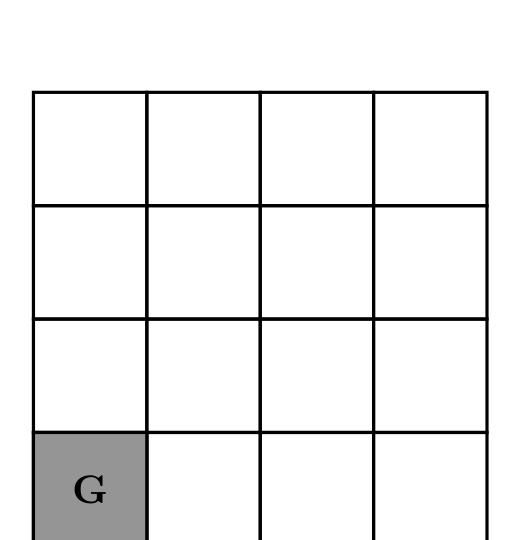
\includegraphics[width=0.22\textwidth]{fig12_5_grid}
\end{frame}

\begin{frame}{Environments: Cheese Maze}
The \textbf{Cheese Maze} is a more complicated two-dimensional grid-world with one goal
state. The agent has 4 actions ($\mathit{up},\mathit{down},\mathit{left},\mathit{right}$)
and 16 observations $\Ocal=\BB^4$: each bit of the observation indicates whether a wall is
directly adjacent to the north, east, south, or west of the agent, respectively.

There are three rewards: $-10$ for bumping into a wall, $+10$ for finding the goal state
(``cheese''), and $-1$ for moving into a state that is not a wall or the goal (to
incentivize finding the cheese quickly). Whenever the agent enters the cheese cell, it is
teleported to a random non-cheese cell.

Since the environment has \emph{partial aliasing}: if the agent starts in a cell and
observes $\mathtt{0101}$, there is not enough information to determine whether the cheese
is directly below, or the agent is in one of the two side corridors -- it needs to move up
and then down to disambiguate and find the cheese.

\centering
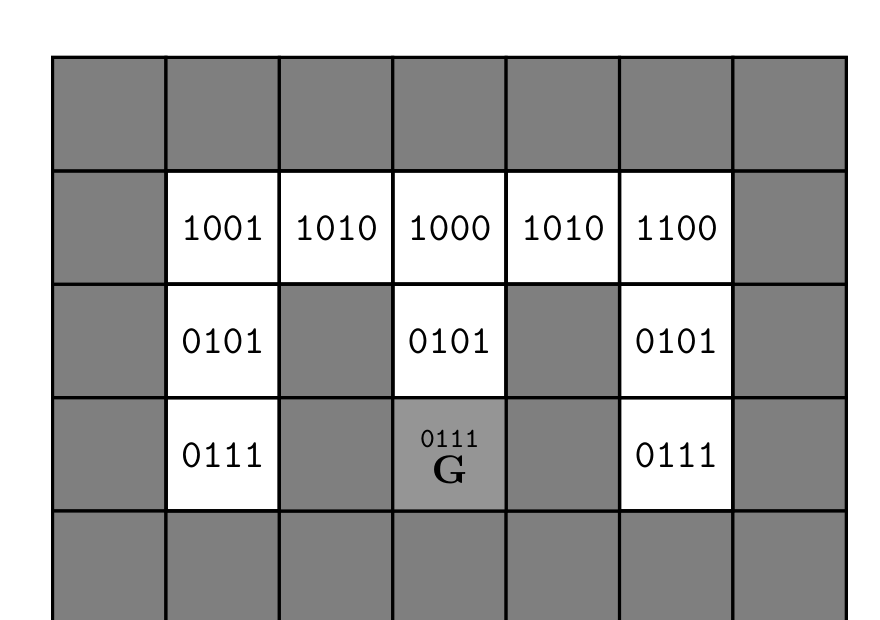
\includegraphics[width=0.40\textwidth]{fig12_6_cheese}
\end{frame}

\begin{frame}{Environments: Tiger and Extended Tiger}
\textbf{Tiger.} The agent faces two doors: behind one is gold, the other a tiger. Three
actions: \emph{listen} (tells the agent which door the tiger is behind, correct with
probability $0.85$), \emph{open door 1}, \emph{open door 2}. Opening a door gives reward
$-100$ if the tiger is found, $10$ if the gold is found. \emph{Listen} gives reward $-1$
(to discourage listening forever, though the agent is not forbidden from doing so). Once a
door is opened, the doors close and are reshuffled.

\textbf{Extended Tiger.} Adds: the agent is either sitting or standing, starting seated.
Two additional actions, \emph{stand up} and \emph{sit down}. The agent can only listen
while sitting, and only open doors while standing. Any illegal action (opening a door
while sitting, standing while already standing, etc.) gives reward $-10$. The reward for
finding the gold is now $30$. The environment resets once any door is opened.
\end{frame}

\begin{frame}{Environments: TicTacToe and Biased RPS}
\textbf{Tic Tac Toe.} The well-known game against an opponent who chooses actions
uniformly at random. The agent has 9 actions: placing a piece in one of the nine squares.
The observation space is the current board state. Reward $2$ for winning, $1$ for a draw,
$-2$ for losing, $-3$ for an illegal move, $0$ otherwise. Illegal moves are punished
\emph{more} than losing to encourage the agent to learn legal moves and prefer losing to
playing illegally.

\textbf{Biased RPS (Rock-Paper-Scissors).} The opponent is \emph{biased}: if they won the
last round playing rock, they choose rock again; otherwise they choose uniformly at
random. The agent needs to learn and exploit this bias. Reward $1$ for winning, $0$ for a
draw, $-1$ for losing.
\end{frame}

\begin{frame}{Environments: Kuhn Poker}
\small
\textbf{Kuhn poker} [Kuh50] is a simplified poker with a 3-card deck: King $>$ Queen $>$
Jack. The opponent plays first, the agent second. Observations are the card held plus the
opponent's actions. Both players \emph{ante} one chip. One betting round: opponent
\emph{raises} (bets another chip) or \emph{checks} (passes). If raised, the agent
\emph{calls} (matches) or \emph{folds} (surrenders). If checked, the agent may raise or
check (to which the opponent must then call or fold). If a player folds, the other wins
the pot minus the chips they staked; otherwise a \emph{showdown} occurs and the higher
card wins the pot. This version is simple enough that a mixed \textbf{Nash equilibrium}
strategy is known for both players -- the opponent plays this Nash strategy, and the
optimal strategy for the agent is also the Nash strategy, giving an average return of
$1/18$ reward per hand.

\centering
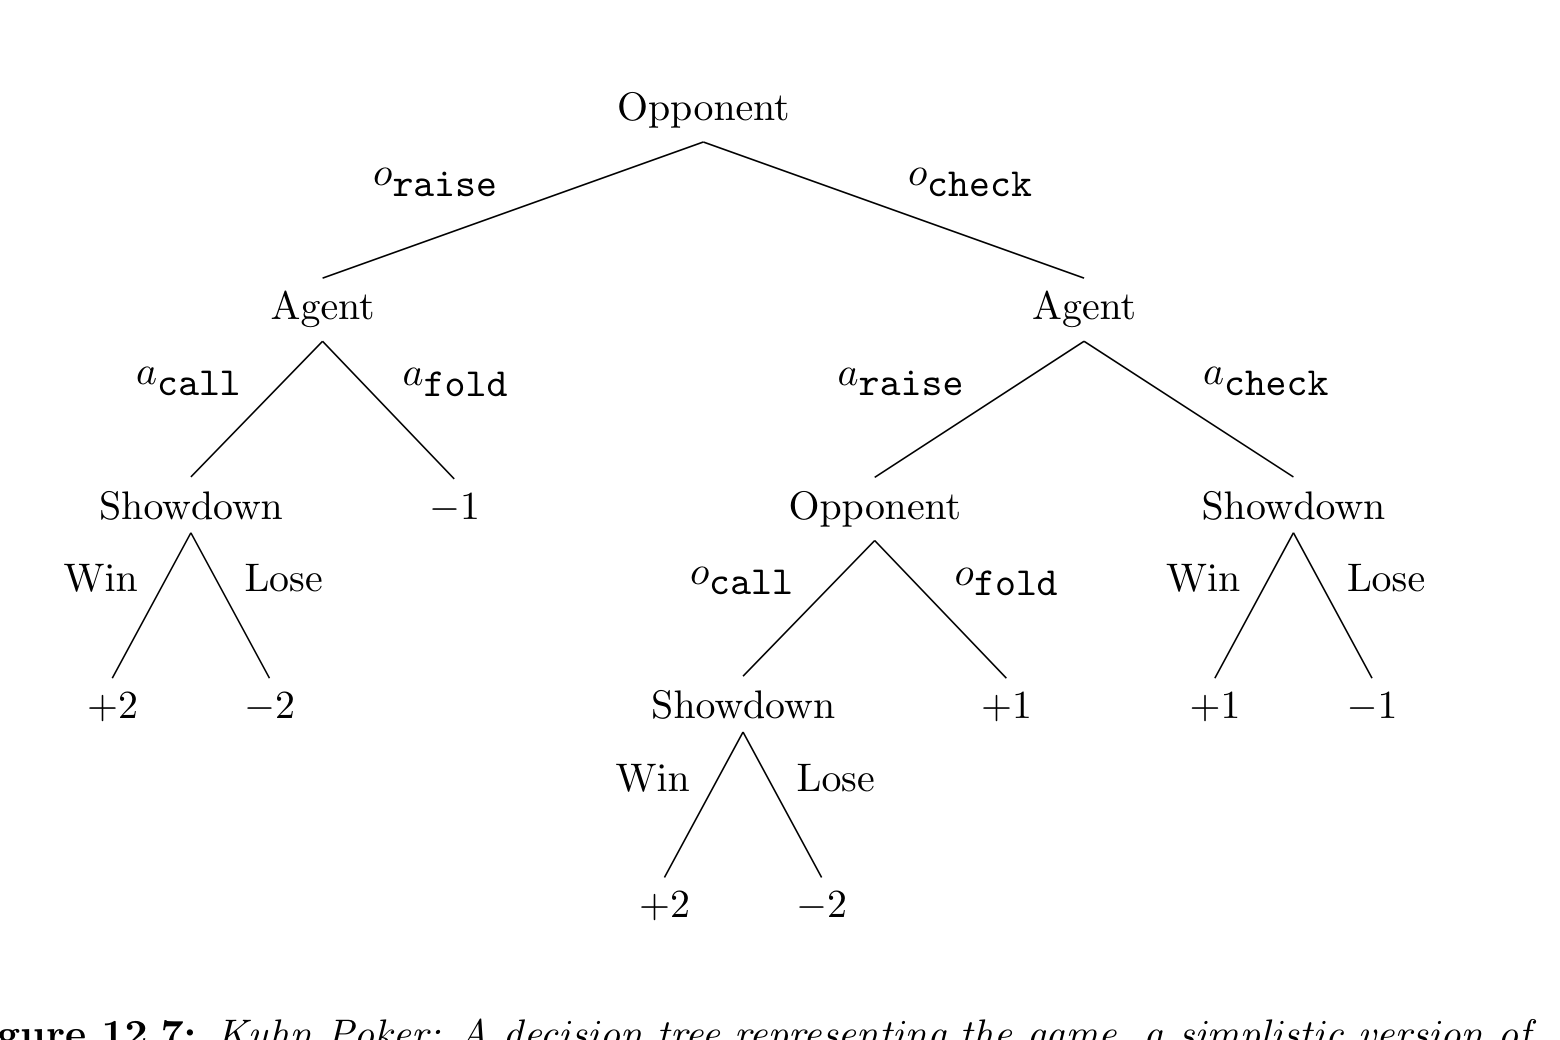
\includegraphics[width=0.52\textwidth]{fig12_7_kuhn}
\end{frame}

\begin{frame}{Environments: POCMAN}
\small
The most complex environment tested is \textbf{POCMAN} [SV10], a partially observable
version of the classic arcade game Pac-Man. The agent navigates a $17\times17$ maze
(Figure 12.8) and eats food pellets. Four ghosts roam the maze: initially at random, but
once within Manhattan distance $5$ of Pac-Man they aggressively pursue for a short
duration. Pac-Man only receives a \textbf{4-bit} observation of the wall configuration at
its current location (as in the Cheese Maze), a 4-bit observation of whether a ghost is
visible (via direct line of sight) in each of the four cardinal directions, a 3-bit
observation indicating whether a food pellet exists within Manhattan distance $2$, $3$, or
$4$, a 4-bit observation of food visible via direct line of sight, and a single bit
indicating whether Pac-Man is under the effect of a power pill (which allows eating ghosts
for the next 100 steps).

\textbf{Rewards:} $-1$ per movement action, $-10$ for running into a wall, $+10$ per food
pellet eaten, $-50$ if killed by a ghost (episode resets), $+30$ for eating a ghost under
a power pill, $+100$ for collecting all the food (cumulative if multiple events occur
simultaneously). The episode resets if the agent is caught or collects all food.

\centering
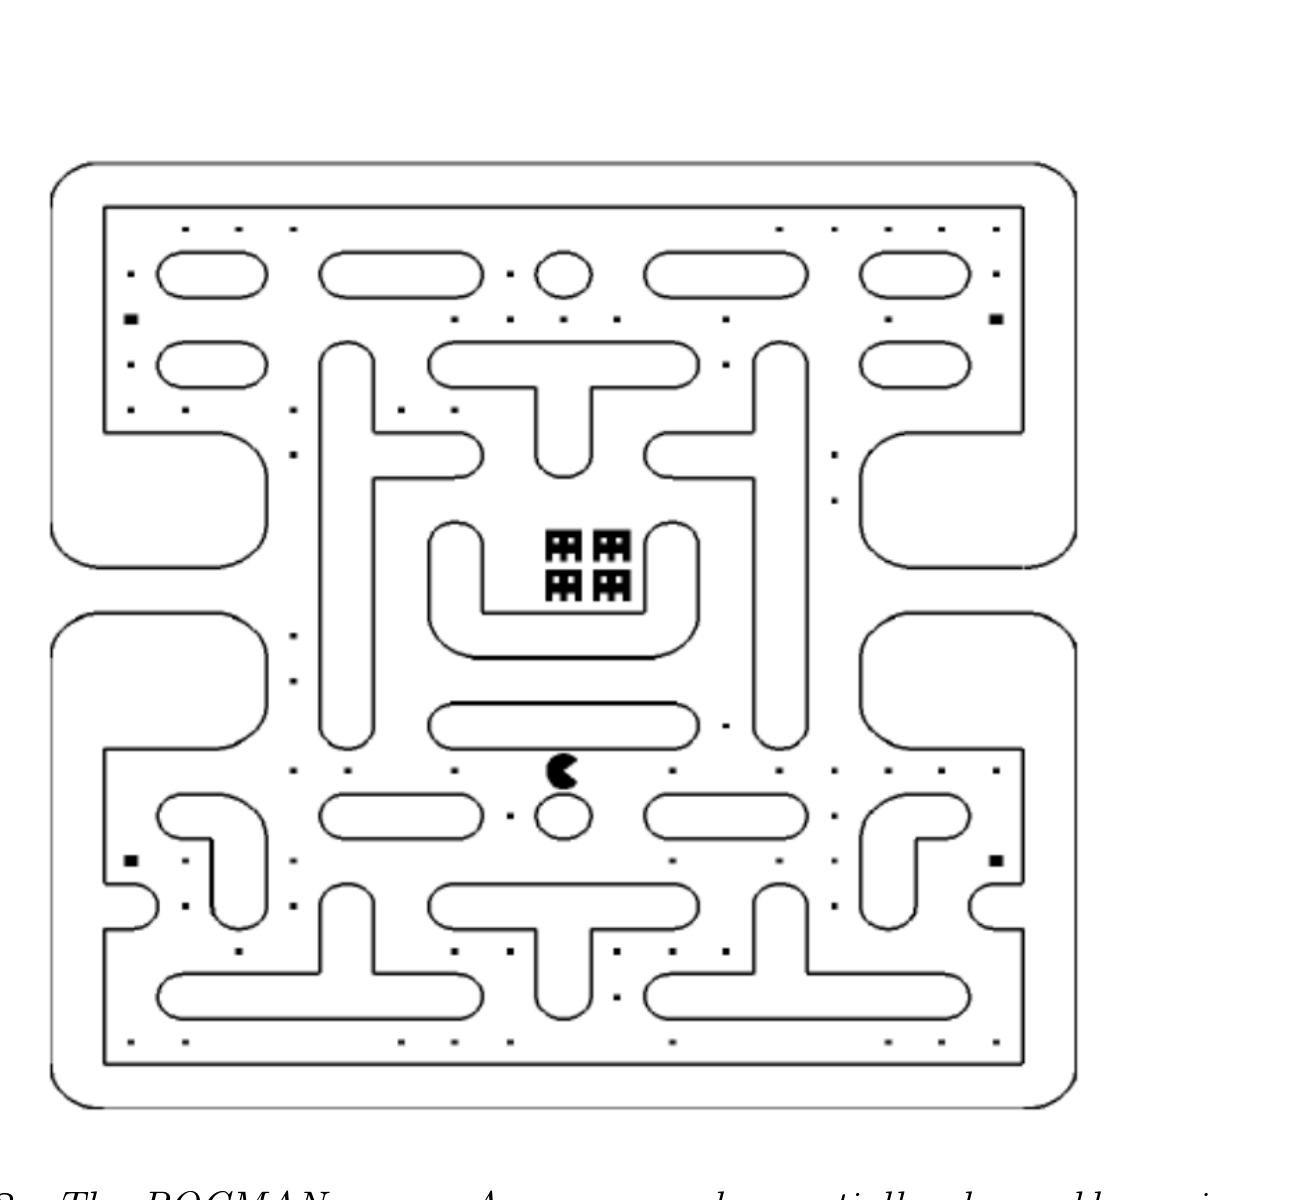
\includegraphics[width=0.34\textwidth]{fig12_8_pocman}
\end{frame}

\begin{frame}{12.5.2 Empirical Performance}
In each environment except POCMAN, [VNHS10] compared MC-AIXI-CTW against two baselines:
\textbf{U-Tree} [UV98] (which learns a compact state representation from the raw history
stream) and \textbf{Active-LZ} [FMRW10a] (which uses a Lempel-Ziv-based prediction scheme
combined with dynamic programming for control). MC-AIXI-CTW outperformed both baselines in
every environment tested.

Figure 12.9 (shown earlier) summarizes performance across environments, with reward
normalized so that an average reward of $1$ per cycle corresponds to the optimal policy.
On every environment except POCMAN, MC-AIXI-CTW eventually learns to play optimally --
POCMAN's much larger state and observation space ($2^{16}$ possible observations) makes
learning slower and full convergence harder to reach within a practical number of
interactions.
\end{frame}

% ============================================================
\section{AIXIjs Implementation}
% ============================================================

\begin{frame}{12.6 AIXIjs: A JavaScript Testbed for AIXI Approximations}
\textbf{AIXIjs} [ALH17, Asl17] is a toy implementation, in JavaScript, of various
approximations of AIXI from Chapters 7, 9, and 12 of this book. It is an easy-to-use
testbed for experimentally comparing (approximations of) AIXI and other universal agents,
such as \textbf{Knowledge-Seeking Agents}, \textbf{BayesExp}, and \textbf{Thompson
sampling}. Several environments are implemented, including various gridworlds and MDPs
[Put14].

AIXIjs has been used to study wireheading in partially embedded agents [MSZ19], the
effects of generalized discount functions [LALH17], and how new universal-AI agents
perform experimentally compared to other UAI agents [CCH19, CHC21].

\textbf{This chapter's comparison} uses two choices of model class over a
$10\times10$ gridworld containing a single reward dispenser (which gives reward with
probability $0.75$): (1) a class of possible reward-dispenser \emph{locations} -- used by
the base AIXI approximation MC-AIXI-CTW; and (2) a Dirichlet distribution over grid cells
the agent can visit -- used by the knowledge-seeking agents (Section 9.3). For the UCT
search, $600$ samples are used with a planning horizon of $6$; each agent's performance is
averaged over $50$ simulations.
\end{frame}

\begin{frame}{Figure 12.10: Knowledge-Seeking Exploration in AIXIjs}
\centering
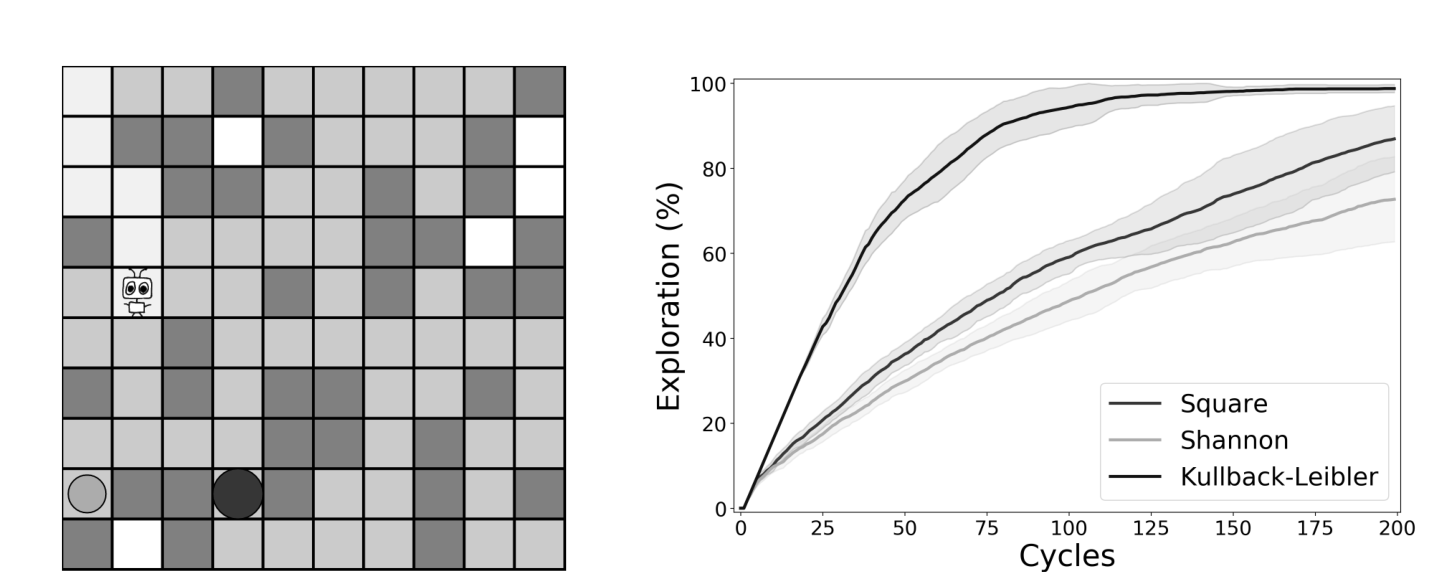
\includegraphics[width=0.78\textwidth]{fig12_10_grid_explore}

\footnotesize (Left) a gridworld in AIXIjs: darker gray indicates a higher belief of
potential reward at that cell. (Right) exploration percentage over time for three
knowledge-seeking agents: \emph{Square}, \emph{Shannon}, and \emph{Kullback-Leibler} (KL).
Performance in terms of intrinsic motivation is highly model-dependent: for the Dirichlet
base model class, the information-seeking (KL) policy outperforms entropy-seeking
(Shannon) in this stochastic environment; the curves for the location-based model class
look similar to Shannon but only reach $\approx75\%$ exploration.
\end{frame}

\begin{frame}{Figure 12.11: MC-AIXI vs.\ Thompson Sampling}
\centering
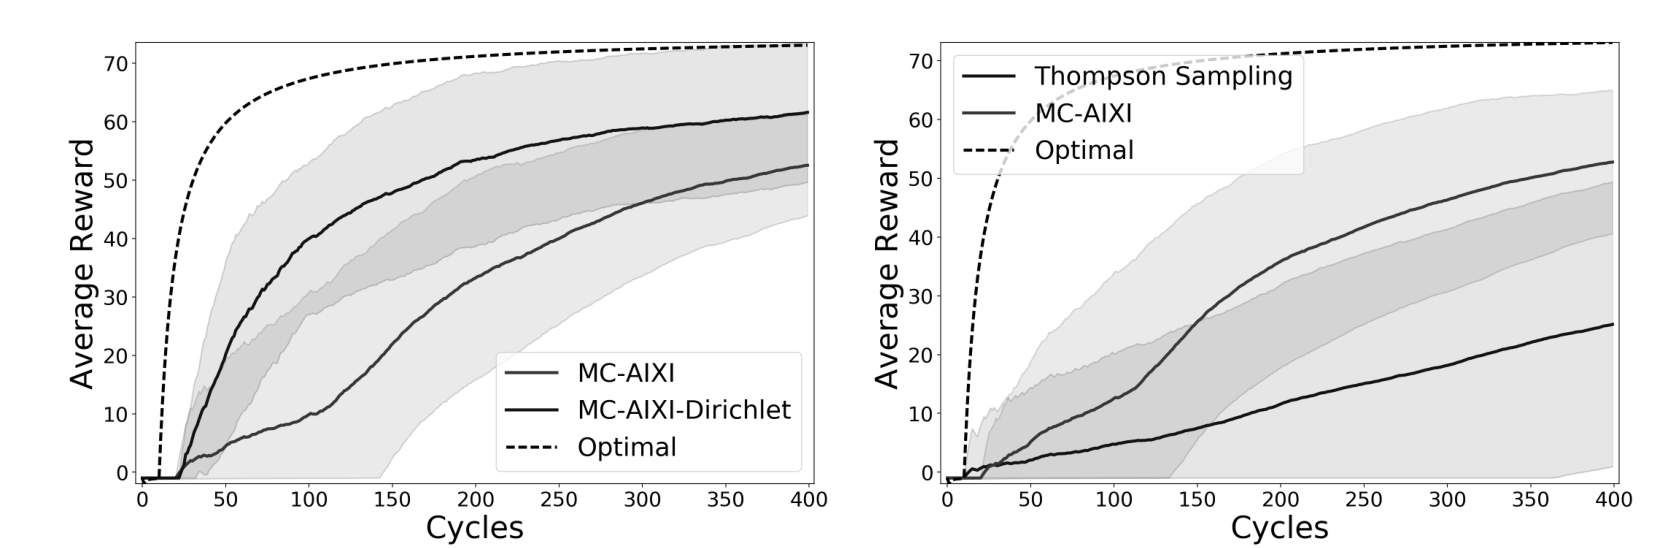
\includegraphics[width=0.78\textwidth]{fig12_11_reward_curves}

\footnotesize (Left) average reward of MC-AIXI using the \emph{location} model class
(thin line) vs.\ the \emph{Dirichlet} model class (thick line), both vs.\ the theoretical
optimum. (Right) MC-AIXI typically outperforms Thompson sampling: both share MCTS horizon
$m=6$ and budget $600$ samples/action, yet Thompson sampling is unreliable, with low mean
reward and high variance (with horizon $10$ and budget $100$, the gap narrows but remains
significant). Interestingly, Thompson sampling is \emph{proven} asymptotically optimal
while MC-AIXI-CTW is not -- likely its extra exploration hurts it in this finite-sample
regime relative to MC-AIXI-CTW.
\end{frame}

\begin{frame}[fragile]{Python: Knowledge-Seeking Exploration Bonuses}
\begin{lstlisting}
# Illustrative (not from the book): compare three intrinsic exploration
# bonuses used by knowledge-seeking agents in AIXIjs, for a simple belief
# update over "is there a reward dispenser in this cell?" (Bernoulli(theta)).
import numpy as np

def square_bonus(p_before, p_after):
    return (p_after - p_before) ** 2

def shannon_bonus(p_before, p_after):        # entropy-seeking (Shannon)
    def H(p):
        p = np.clip(p, 1e-9, 1 - 1e-9)
        return -(p * np.log(p) + (1 - p) * np.log(1 - p))
    return H(p_after) - H(p_before)

def kl_bonus(p_before, p_after):             # information-seeking (KL)
    p_before = np.clip(p_before, 1e-9, 1 - 1e-9)
    p_after = np.clip(p_after, 1e-9, 1 - 1e-9)
    return p_after * np.log(p_after / p_before) + \
           (1 - p_after) * np.log((1 - p_after) / (1 - p_before))

p_before = 0.5                 # uniform prior belief
p_after = 0.9                  # after observing strong evidence of a dispenser
for name, fn in [("Square", square_bonus), ("Shannon", shannon_bonus), ("KL", kl_bonus)]:
    print(f"{name:8s} bonus = {fn(p_before, p_after):+.4f}")
# Square  bonus = +0.1600
# Shannon bonus = -0.2081   (surprisingly negative: entropy *decreased*)
# KL      bonus = +0.5108   (KL divergence is always non-negative)
\end{lstlisting}
\end{frame}

% ============================================================
\section{Discussion}
% ============================================================

\begin{frame}{12.7 Discussion}
\begin{itemize}
\item The Monte Carlo AIXI Context-Tree-Weighting (MC-AIXI-CTW) agent represents the
initial attempt to approximate AIXI in a way that scales to more complex environments than
the exhaustive-search AIXI-MDP agent of Chapter 11.
\item By employing the CTW method, $\xi_{FAC}$ constructs an \emph{efficient} Bayesian
mixture, yielding a manageable version of AIXI's mixture $\xi$ -- turning a
double-exponential intractability into an $O(D)$-per-bit update.
\item As discussed in Chapter 5, various extensions of CTW have been proposed, each
enhancing different aspects of the original method (handling different context
structures, different priors, etc.). These improvements can be readily integrated into the
MC-AIXI-CTW framework, replacing the original CTW component and potentially improving the
agent's overall performance.
\item Together, MCTS (searching) and CTW (learning) show that both halves of the AIXI
equation -- planning given a model, and learning a model from data -- admit efficient,
practical approximations, and that combining them yields an agent that performs well
across a strikingly diverse range of environments, entirely from scratch.
\end{itemize}
\end{frame}

% ============================================================
\section{Exercises}
% ============================================================

\begin{frame}[allowframebreaks]{12.8 Exercises}
\begin{enumerate}
\item[1.] [C07] Assume a bandit problem has a unique optimal action $a^*$. Prove that an
$\varepsilon$-greedy agent converges to a policy that chooses $a^*$ with probability
$1-\varepsilon\big(1-\tfrac1{|\Acal|}\big)$.
\item[2.] [C25] In UCT, derive the worst-case-regret bound of using $\ln^2 N(h)$ or
$\sqrt[3]{N(h)}$ (or other functions in $o(\sqrt{N(h)})$). How do they compare to the
bound of $\ln N(h)$?
\item[3.] [C30] Prove Theorem 12.2.6.
\item[4.] [C15] Run an experiment comparing the performance of BayesExp and Thompson
sampling agents in gridworlds on the AIXIjs website.
\item[5.] [C12] Prove that we can always apply a positive affine transformation to the
rewards to ensure they are always non-negative, without changing the optimal policy. See
also Exercise 15.5.
\item[6.] [C25] Implement $\rho$-UCT together with FAC-CTW to replicate MC-AIXI-CTW, and
graph the performance against each environment (Figure 12.9). A reference implementation
can be found at \texttt{https://jveness.info/software/default.html}.
\item[7.] [C25] Investigate why leaf parallelization performs poorly compared to other
methods for parallelizing MCTS (Section 12.2.6).
\item[8.] [C28] Investigate the extensions of CTW (Chapter 5) and use them in place of CTW
to define $\xi_{FAC}$. Does this improve the MC-AIXI-CTW model?
\item[9.] [C20] Train MC-AIXI-CTW on a simple environment (e.g.\ 1D Maze or Tiger) and
then continue on another simple environment. Does MC-AIXI-CTW perform better or worse on
the second domain? Repeat with different pairs of environments.
\item[10.] [C18] For the UCT action selection, test alternative choices of the constant
$C$. Show that if $C$ is sufficiently large UCT will fail.
\item[11.] [C20] Use the CTW algorithm to learn a fast approximation of the policy and
use it for the rollout in $\rho$UCT. What is gained/lost by using this in place of a
random policy?
\item[12.] [C32] Prove Theorem 12.4.1.
\item[13.] [C25] Generalize FAC-CTW to $\mathcal{P}$-context trees defined in Section 9 of
[VNH$^+$11].
\end{enumerate}
\end{frame}

% ============================================================
\section{History and References}
% ============================================================

\begin{frame}{12.9 History and References (1/5)}
This chapter is primarily based on [VNH$^+$11], where CTW (for learning) and the UCT
algorithm (for planning) are first combined. In [BVB13], an agent was constructed for
Atari 2600 games by recursively factoring the large observation space into smaller,
manageable sub-problems, with a Bayesian average taken over the result -- working
similarly to CTW. [VSH12] surveys possible ways to extend CTW, particularly for the active
(reinforcement learning) case; FAC-CTW, introduced in [VNHS10], is one novel example. The
AIXIjs testbed was developed in [Asl17, ALH17], with various approximations of AIXI
discussed in this book and various toy environments implemented.

\textbf{AIXI approximations.} Several other attempts have been made to study the
computational properties of AIXI:
\begin{itemize}
\item AIXI$tl$ [Hut05b, Chp.\,7] (Section 13.2) uses the best policy, as measured by a
provable lower bound on the value function, bounded in space $l$ and time $t$. It is
based on the provably fastest algorithm for all well-defined problems [Hut01b, Hut02b],
related to \textbf{Levin Search} [Lev73c], which solves any inversion problem optimally
within multiplicative overhead but is impractical in general (though can be applied
successfully in some cases [Sch97b, SZW97, Sch03, Sch04]).
\end{itemize}
\end{frame}

\begin{frame}[allowframebreaks]{12.9 History and References (2/5)}
\small
\begin{itemize}
\item \textbf{Self-AIXI} [CGMH$^+$23] (Section 9.5) is a modification of AIXI that avoids
planning by self-predicting its own actions; its practical instantiation Self-AIXI avoids
the expensive MCTS used in MC-AIXI-CTW.
\item In domains with very small action/percept spaces and restrictive assumptions on the
model class, universal learning is computationally feasible via brute-force search
[PH06b] (Chapter 11). The behavior of AIXI-MDP is compared with a universal
predicting-with-expert-advice algorithm [PH05b] in repeated $2\times2$ matrix games, and
shown to exhibit different behavior.
\item In [Pan08], a Monte Carlo algorithm samples from a time-bounded version of the
universal Solomonoff prior. A closely related algorithm samples from a \textbf{speed
prior} [Sch02b, FLH16], a universal semimeasure like the Solomonoff prior that also
considers the number of time steps needed to compute a result.
\item \textbf{$\Phi$-AIXI-CTW} [YZWN22] (Chapter 14) abstracts the complete history (as in
Chapter 14) and then applies CTW to the abstracted history, enabling environment model
classes with arbitrary dependence on the history.
\item \textbf{DynamicHedgeAIXI} [YZNH24] dynamically adds (and subtracts) models via a
time-adaptive prior built from a variant of the Hedge algorithm -- the latest and richest
direct approximation of AIXI at time of writing, with good theoretical and practical
guarantees.
\item An alternative approach to approximating Bayes-optimal agents like AIXI was
developed in [MDM$^+$20], where it was shown that \emph{meta-training} can approximate
Bayes-optimality.
\end{itemize}
\end{frame}

\begin{frame}{12.9 History and References (3/5): UCB, MCTS, USM/U-Tree}
\textbf{Upper Confidence Bounds and Monte Carlo Tree Search.} UCB was first introduced in
[ACBF02]; it has since been extended to contextual bandits [LS20, Part V] with linear,
non-linear, and gated linear function approximation [SHB$^+$20]. Extending UCB from
bandits to MDPs (i.e.\ UCT) was done in [KS06]. UCB has had many successful practical uses,
including the game Go [GW06], and learning to play new games from a provided description
of the rules [FB08]. [GS07] modified UCB to combine online-learned statistics with offline
learning via TD($\lambda$). Improvements to the rollout stage of MCTS include a 1-ply
rollout-based planning technique for noisy stochastic domains [BC99], knowledge-based
rollout policies in Go [GWMT06], and learning the rollout policy for adversarial games
[ST09]. MCTS was used to adjust a heuristic for chess game-tree search [VSBU09]. For large
partially observable domains, the \textbf{POMCP} algorithm combines the agent's belief
state with MCTS from the state the agent believes itself to be in [SV10].

\textbf{USM and U-Tree.} An early influential work is the \textbf{Utile Suffix Memory}
(USM) algorithm [McC96], which partitions the agent's history space into distinct states,
one per leaf of a suffix tree, each with an associated Q-value updated incrementally
much like Q-learning [WD92]. The suffix tree grows incrementally, splitting a leaf when
its history sequences show statistically different Q-values; USM does not deal
effectively with noisy environments (extensions in [SB04, Sha07]).
\end{frame}

\begin{frame}{12.9 History and References (4/5): U-Tree, Universal RL, BLHT}
\textbf{U-Tree} [McC96] is an online agent algorithm that discovers a compact state
representation from raw experience. Unlike USM, U-Tree can discriminate between
\emph{individual components} within an observation, letting it handle larger observation
spaces and ignore irrelevant components. Each state is a leaf of a suffix tree mapping
history sequences to states; the representation is refined via a heuristic built around
the Kolmogorov-Smirnov test [BZ14], limiting the tree's growth to nodes that improve
future-reward prediction. Value iteration updates the value function at each time step.

\textbf{Universal RL.} \textbf{Active-LZ} [FMRW10a] combines a Lempel-Ziv-based prediction
scheme [ZL77] with dynamic programming for control, producing an agent provably
asymptotically optimal in $k$-Markov environments. It builds a context tree (distinct from
the CTW context tree) with accumulated transition statistics and a value-function
estimate at each node, refined over time. MC-AIXI-CTW compares favorably to Active-LZ
[VNH$^+$11, Sec.\,7].

\textbf{Bayesian approach to Learning History Trees (BLHT)} [SHL97, SH98] uses symbol-level
PSTs for learning and dynamic programming for control. BLHT uses the \textbf{MAP}
(maximum a posteriori) model for prediction, as opposed to CTW's full Bayesian mixture,
which admits a much stronger convergence result; CTW's prior also weights models by
complexity (Occam's razor), instead of the uniform prior over PST models used by BLHT.
\end{frame}

\begin{frame}[allowframebreaks]{12.9 History and References (5/5): PSRs, MBRL, CnC, Quantum AIXI}
\small
\textbf{Predictive State Representations (PSRs)} [LS01, RGT04, SJR12] maintain predictions
of future experience as a vector of probabilities for the outcomes of various
\emph{tests} (predicates about future observations given particular action sequences). If
every test's outcome were known, the environment's dynamics would be known; a PSR is a
sufficient subset of these predictions. Exact PSRs are impractical in large domains, so
approximation is typically required (e.g.\ kernel-based PSRs [BSG11]; temporal-difference
networks [ST04], where an \emph{answer network} predicts future observations and is
updated via temporal-difference learning). In model-based Bayesian RL [Str00b, PVHR06,
RCdP07, PV08], a distribution over (PO)MDP parameters is maintained; in contrast, MC-
AIXI-CTW maintains an \emph{exact} Bayesian mixture of PSTs.

\textbf{Compress and Control (CnC)} [VBH$^+$15, DRW$^+$24] decomposes the distribution of
the return $z$ (rather than predicting observations/rewards one step at a time) via
$\rho(z|s,a)\stackrel{\triangle}{=}\rho(s|z,a)\rho(z|a)$; using CTW leads to consistent
estimation [VBH$^+$15]. This is a compression-based method for both policy evaluation and
on-policy control.

\textbf{Quantum AIXI.} [CH20a] first tackled whether quantum computing can speed up
approximations of Solomonoff induction and AIXI; speedups were found but not the
exponential speedup quantum computing achieves elsewhere. [Sar21, SAAGB21] instead
consider a model class of \emph{quantum-computable} (semi)measures, defining a
Knowledge-Seeking Agent (Section 9.3) variant over this model class.

\textbf{Related approximations \& AI search.} Compress and Control, Representational MDL
[PR12], Feature Reinforcement Learning (Chapter 14), and low-Kolmogorov-complexity policy
search [SJ21] all embody the spirit of UAI without being direct AIXI approximations. MCTS
[KS06] is one instance of the long tradition of AI search: (iterative-deepening)
A$^*$ [HNR68, Kor85], breadth-first search [Zus72], depth-first search [Tre76] (see
[EH15a, EH15b] for a comparison), and Levin (tree) search [OHL23], among many variants.
\end{frame}

\begin{frame}{Chapter Summary}
\begin{itemize}
\item \textbf{Searching}: exact expectimax is intractable ($O(|\Acal\times\Ecal|^m)$);
\textbf{Monte Carlo Tree Search} approximates it via sampled rollouts, guided by
\textbf{UCB}-style action selection (\textbf{UCT}) that provably converges and provably
requires the $\ln N(h)$ exploration term to avoid getting permanently stuck.
\item \textbf{Learning}: the exact AIXI mixture $\xi$ over all semicomputable environments
is intractable; \textbf{CTW} computes an analogous mixture over context trees in $O(D)$
time. Extending CTW to actions (\textbf{AC-CTW}) and factoring it per percept bit
(\textbf{FAC-CTW}) preserves type information the agent needs to tell rewards from
observations.
\item \textbf{Putting it together}: instantiating $\rho$UCT with $\rho=\xi_{FAC}$ gives
\textbf{MC-AIXI-CTW}, a practical, efficiently computable approximation of AIXI with a
formal error bound (Theorem 12.4.1) and strong empirical performance across a wide range
of POMDP-style environments -- from simple mazes to Kuhn poker to POCMAN.
\item MC-AIXI-CTW is not the final word: $\Phi$-AIXI-CTW, DynamicHedgeAIXI, Self-AIXI, and
meta-trained approximations all push further along the same basic recipe of
\emph{tractable learning} $+$ \emph{tractable search} $\approx$ AIXI.
\end{itemize}
\end{frame}

\end{document}
